\documentclass[usegeometry=true]{scrartcl}
\usepackage[ngerman]{babel}
\usepackage[T1]{fontenc}
\usepackage{lmodern}
\usepackage[utf8]{inputenc}
\usepackage{hyperref}
\usepackage{amssymb}
% Dimensionen bitte nicht ändern. 
\usepackage[left=2cm, right=2cm, top=2cm, bottom=2cm, bindingoffset=1cm, includeheadfoot]{geometry}
%Zeilenabstand bitte nicht ändern
\usepackage[onehalfspacing]{setspace}
%grafik einfügen
\usepackage{graphicx}
%arbeiten mit mehreren Bilder
\usepackage{subfigure}
%einfügen von hyperref
\usepackage{hyperref}
%nested imtemize
\usepackage{enumitem}
\usepackage[backend=biber,style=numeric,]{biblatex}\addbibresource{literatur.bib}

\begin{document}
% ----------------------------------------------------------------------------
\subject{Projektbericht zum Modul Information Retrieval und Visualisierung Sommersemester 2022}
\title{Visualisierung des Datensatzes Student Behaviour}
%\subtitle{Untertitel}% optional
\author{Paul Tebbe, Matrikelnummer: 216237588}% obligatorisch
\date{21.12.2022}

\dedication{\normalsize\vfill\hrule\vspace{10pt}
	Link zum GitLab-Repository:\\
	\url{https://github.com/TornadoTebbe/Elm-Visualisation}\\
	
	\vspace{10pt}
	Link zur öffentlich zugänglichen Webseite (GitLab Pages):\\
	\url{https://tornadotebbe.github.io/}
}


\maketitle% verwendet die zuvor gemachte Angaben zur Gestaltung eines Titels
\pagebreak
% ----------------------------------------------------------------------------
Inhaltsverzeichnis:
\tableofcontents
% ----------------------------------------------------------------------------
% Gliederung und Text:

\section{Einleitung}
\label{Einleitung}

Viele verschiedene Faktoren haben einen Einfluss auf die Note der Studenten. Dies geht bereits damit los in welche Familie das Kind hineingeboren wird, welchen akademischen Standard die Eltern haben, welche finanziellen Mittel usw. Weiter spielt die Erziehung und der spätere soziale Umgang eine Rolle. \cite{Earthman}
Diese Einflüsse sind schwer zu messen, vor allem schwer genau zu messen. Zudem sind diese Faktoren kaum von alleine beeinflussbar.\\
Doch auf welche Faktoren kann der Student selber später Einfluss nehmen. Die Zeit, die täglich in oder eben nicht in die schulische Weiterbildung investiert wird, sollte in der Theorie so einen selbst beeinflussbaren Faktor darstellen. Und ich welcher weise lässt sich auch eine Tendenz Tendenz in der Fluktuation der Noten erkennen. Bleiben Schüler, die bereits in der Schule schlechtere Noten haben auch im College schlecht?
In dieser Arbeit werden sich also folgende Fragen und folgende gestellt Zielstellungen gesetzt:

\begin{itemize}
\item Wie korrelieren Noten und Zeitgestaltung und lassen sich daraus Rückschlüsse ziehen, wenn ja welche? 
\item Wie stehen die Noten im Zusammenhang mit anderen Variablen?
\item Wie können die verschiedenen Daten übersichtlich veranschaulicht werden um dem Leser einen schnellen Überblick zu geben
\end{itemize}



Tipps zu Latex und Koma-Script für Hausarbeiten sind im \href{http://mirrors.ctan.org/info/latex-refsheet/LaTeX_RefSheet.pdf}{LaTeX Reference Sheet for a thesis with KOMA-Script} von Marion Lammarsch und Elke Schubert zusammengefasst. 
Der Bericht fällt in die Kategorie von InfoVis-Paper, die Tamara Munzner Design Study nennt \cite{Munzner2008}: In der Einleitung sollen sie zuerst das Zielproblem beschrieben. Daraus sollen sie Fragestellungen motivieren, die mittels Techniken der Informationsvisualisierung beantwortet werden können. In dem Abschnitt direkt unter der Überschrift Einleitung sollen Sie nach einer kurzen Einleitung Fragestellungen und das Zielproblem motivieren und beschreiben. ...

\subsection{Anwendungshintergrund}
Wer in der Schule und im College gute Noten hat und sich somit einen besseren Abschluss erarbeitet hat im späteren Leben deutlich bessere Chancen auf \glqq individuelle Lebenschancen, Selbstverwirklichung, beruflichen Erfolg sowie soziale, politische und kulturelle Teilhabe. \grqq
%\citep{Solga, Dombrowski 2008}





\subsection{Zielgruppen}
Die Zielgruppe für die Daten umfasst ein weites Spektrum an Personen. Die Visualisierung sind sowohl für Schüler und Studenten, als auch für Lehrer und Eltern interessant, also jegliche Personengruppe, die Berührungspunkte mit der Notengebung und deren Einflussfaktoren aufweist.
Die Informationen, die aus den Visualisierungen gewonnen werden können, können sehr gut dafür genutzt werden zu sehen, wie grade der Einflussfaktor Lernzeit und auch die vorangegangen Noten aus der Schulzeit einen Einfluss auf die Noten im College nehmen. Differenziert werden kann hierbei auch nochmal unter den Geschlechtern. 
Auch interessant könnte dieses Projekt aber auch für Forschende im Bereich soziale Ungleichheiten in der Bildung sein. Wenn keine eindeutigen Anzeichen zu sehen sind für eine Korrelation zwischen investierter Lernzeit und besseren Noten, so könnte dies ein Anzeichen dafür sein, dass doch andere Einflussgrößen mehr Auswirkung auf die Noten haben als der reine Fleiß. Dies wäre ein starker Indikator für soziale Ungleichheiten bei der Bildung, wie es bereits in der Einleitung angedeutet wurde. 


\subsection{Überblick und Beiträge}
Der in dieser Arbeit verwendete Datensatz differenzieren die Studenten nach verschiedenen Merkmalen. Diese gehen von allgemeinen Unterscheidungen, wie Geschlecht, Alter und Gewicht, über die Aufteilung ihrer Freizeit und die aufgewendete Lernzeit bis hinzu dem körperlichen Wohlbefinden ausgedrückt mittels der Variable \glq stress level \grq .



\noindent Die für diese Visualisierung mit am interessantesten Daten sind die der verschiedenen Noten in der Schule und im college. Die Noten, gerade mit der von den Studenten angegebenen täglich Lernzeit sollte in einem positiven Zusammenhang stehen. Also steigt die Lernzeit am Tag, steigt auch die Note. Das gleiche sollte auch für die Beziehung der Noten untereinander gelten, also welcher Student schon in der 10.ten und 12.Klasse gute Noten hatte, sollte nun auch im College gut abschneiden. 
\noindent Die körperlichen Voraussetzungen sowie das Department sollten eigentlichen keine größeren Einflüssen auf die Noten haben.
\noindent Die Zeit verbracht auf sozialen Medien könnte eine negative Korrelation mit den Noten aufweisen, genauso wie der finanzielle Status und das Stress Level bei den Studenten.

In diesem Abschnitt geben sie einen kurzen Überblick über die Daten und verwendeten Visualisierungen. Dann benennen sie die Beiträge ihres Projekts. Diese Beiträge müssen sie in den hinteren Teilen des Berichts genauer ausführen und belegen.

\section{Daten}

Wie bereits in den Abschnitten vorher erwähnt, handelt es sich bei den vorliegenden Daten um den Datensatz \textit{Student Behaviour} von \textit{kaggle} . Die darin aufgeführten und gesammelten Daten geben nähere Auskunft über das Verhalten der Studenten und deren Noten. Die Verwendung des Datensatzes zu wissenschaftlichen Zwecken ist abzuraten, da der Verfasser angibt die Daten selber von Universitäten gesammelt zu haben und bis auf diesen Satz keine näheren Informationen zur Datenbeschaffung liefert. Seiner Meinung nach kann der Datensatz dazu genutzt werden das Verhalten der Studenten in Zukunft besser zu deuten.\\
Im Datensatz auf \textit{kaggle} sind ein paar Rechtschreibfehler bei der Variablenbenennung enthalten, wie z.B. \glqq social medai time\grqq , diese werden daher der Leserlichkeit halber im Folgenden grammatikalisch korrekt geschrieben)
\\
Er enthält Informationen von 235 Studenten in Form einer CSV-Datei. Diese CSV-Datei hat 19 Spalten mit den Informationen der Studenten über \textit{Certification} als Boolean, der ausgibt ob der Student einen certification Kurs besucht hat oder nicht, \textit{Gender} mit Boolean über das Geschlecht, \textit{Department}, welcher Student welchem Derpartment angehört, \textit{Height(CM)} und \textit{Weight(KG)} als Float, die Größe und Gewicht aufzeigen, \textit{10th Mark}, \textit{12th Mark} und \textit{College Mark}, die als Float die Note der Studenten zeigen, \textit{Hobbies}, sowie \textit{stress level} und \textit{financial status} als String, \textit{part-time job} und \textit{Do you like your degree} als Boolean, \textit{salary expectation} als integer (in Elm allerdings als Float deklariert und verwendet, damit es passend visualisiert und gemapt werden kann), \textit{willingness to pursue a career based on their degree } als String in Form einer Prozentangabe (möglich sind hier nur die Angaben: 0,25,50,75 und 100 Prozent) und \textit{travelling time}, \textit{social media time} und \textit{daily studying time} als String in Form einer Klassenangabe (also z.B. 30-60 Minuten ist eine Angabe).

Während sich grade die Noten, also 10th Mark, 12th Mark und College Mark sehr gut dazu eignen die Fragestellung zu beantworten und sich zusätzlich dazu noch gut visualisieren lassen, da sie als Float sich relativ einfach veranschaulichen lassen ist dies bei anderen Variablen weniger der Fall. Bei ein paar der Daten ist nichteinmal genau klar, was damit überhaupt ausgesagt werden soll, wie z.B. bei Certification Course. Was für ein Kurs ist das,  was zertifiziert man damit, bzw. welche Art von Zertifikation erwirbt man damit. Aufgrund des fehlenden Hintergrundwissen, welches leider im Datensatz nicht näher erläutet wird, kann bei diesen Visualisierungen nicht näher darauf eingegangen werden. Ähnlich verhält es sich bei Department. Auch hier fehlen die nötigen zusätzlichen Informationen, um diese Variable in geeigneter Weise einbauen zu können.
Auch die meisten Boolean (part-time job, Do you like your degree,  werden bei den Visualisierungen nicht berücksichtigt (bis auf gender), da es sich, bei den hier verwendeten Darstellungen nicht anbietet boolsche Werte zu integrieren. Diese bieten schlichtweg zu wenige Möglichkeiten.
Vielseitig genutzt wurde auch die daily studying time, die sich vor allem als \textit{drop-down} zur Sortierung der Noten eignete, sodass schnell ersichtlich wurde mit welcher Lernzeit welche Noten erreicht wurden. 
Hier wurde also eine der oben gestellten Zielstellungen sinnvoll und gut umgesetzt.

\subsection{Technische Bereitstellung der Daten}
\label{Bereitstellung}

Die Daten wurden als einzelne CSV-Datei in \textit{kaggle} bereitgestellt und auch also solche weiterverarbeitet. 
Zudem wurden sie im eigenen Github hochgeladen und dort im Ordner Daten gespeichert. Mithilfe dieser Datei wurden der Scatterplot und der Parallelplot erstellt. zur Visualisierung des Baumdiagramms wurde zusätzlich eine json-Datei erstellt \textit{"json.Name"} und auch im Ordner Daten hinterlegt. Zusätzlich dazu finden sich im Github-Repository auch noch Python-Code, mit dessen Hilfe die Daten aufbereitet werden sollen, genaueres in \ref{Datenvorverarbeitung}


\subsection{Datenvorverarbeitung}
\label{Datenvorverarbeitung}
Im obigen Abschnitt wurde bereits kurz auf den Datensatz eingegangen und erklärt, dass es sich um eine einzelne CSV-Date handelte. Aufgrunddessen musste keinerlei größere Vorverabeitung an den Daten vorgenommen werden, zumindest für den Parallelplot und den Scatterplot. Die einzige Datenmanipulation, die hier erfolgte ist die Ausreißerbereinigung. Es gab ein paar wenige extreme Ausreißer (bei \textit{salary expectation}), die dazu führen würden, dass die Visualisierung der Daten darunter leidet. Für diese wurde daher der vorher berechnete Mittelwert eingesetzt.\\

\noindent Für das Baumdiagramm wurde zuerst versucht mithilfe von Pyhtoncode die csv-Datei in eine json-Datei umzuwandeln. Leider gelang dies nicht, sodass die csv erst in eine Excel-Datei umgewandelt wurde. Anschließend wurde mithilfe der Excel-Datei manuell eine json-Datei erstellt um anhand dieser die Baumdarstellung zu visualisieren. In der json wurden dann nur die für das Baumdiagramm relevanten Daten übernommen. Aufgrund anfänglicher Überlegungen die verschieden klassierten \textit{Zeiten}, wie \textit{daily studying time}, \textit{social media time} und \textit{travelling time} in einzelne Klassen in Form von Integers festzuhalten, also \textit{daily studying time} von 0-30 Minuten wäre 1, 30-60 Minuten 2 usw. wurde die csv-Datei in R geladen um die Daten somit zu manipulieren. Aufgrund der späteren Nutzung der \textit{daily studying time} als Drop-down Tabelle wurde dieser Gedanke wieder verworfen.
Für das Baumdiagramm wurden außerdem der Mittelwert der Noten in den jeweiligen Lernklassen berechnet.
Dieser und der vorher für die Ausreißer berechnete Mittelwert sind in der \textit{Student\_Behaviour} Csv-Datei abgespeichert.
\\

\section{Visualisierungen}
\label{gross3}
In den nachfolgenden Abschnitten wird näher auf die oben genannten Zielstellungen eingegangen.

\subsection{Analyse der Anwendungsaufgaben}
Wie bereits in \ref{Einleitung} erwähnt, sollen die folgenden Visualisierungen der Zielgruppe dabei helfen sich einen schnellen und übersichtlichen Eindruck über den Zusammenhang der unterschiedlichen Noten und anderen Variablen machen. Also welche Variablen nehmen möglicherweise Einflüsse auf die Note oder stehen in einem Zusammenhang mit diesen. 
Die Leser:innen  sollen sehen können, wie sich die Noten verändern wenn sich gewisse Variablen verändern, also wie ändert sich die Notenverteilung, wenn sich die Lernzeit erhöht oder verringert, welche Individuen der Ausgewählten sind Männer, welche Frauen. Auch auf einen möglichen Zusammenhang der sich im Laufe der Zeit verändernden Noten soll mithilfe der Visualisierungen eingegangen werden. Sind Studenten, die in der 10. Klasse gute Noten hatten auch in der 12. Klasse und im College noch so gut und umgekehrt genauso: War ein Student mit schlechten Noten schon in der 10. und der 12. Klasse schlecht und hängen diese Dinge möglicherweise mit dem Lernaufwand zusammen. All diese Fragen können in anschaulicher und so auch schneller Art und Weise von den Beobachtern auf den unterschiedlichen Visualisierungen überblickt werden, mit Unterstützung von verschiedenen Drop-Down-Möglichkeiten und der Hover-Funktion (hier werden den Lesern in den Plots immer die Auskunft über das Geschlecht und in manchen Fällen noch weitere allgemeine Informationen geliefert) über den Punkten oder den Parallellinien.
Das normale mentale Modell, dass bei einem Menschen entstehen sollte, wenn er sich diese Fragen und Anwendungsaufgaben stellt ist, dass es eine positive Korrelation zwischen guten Noten in der Schule und guten Noten im College, als auch zwischen Lernzeit und guten Noten existiert. In den Köpfen der Anwender entsteht also ein stetiger Anstieg der durschnittlichen Notenverteilung, je mehr Lernzeit dazukommt und dies sollte auch in den Abbildungen zu sehen sein. Die Mentalen Modelle sind für die Verständlichkeit der Visualisierungen für Leser allerdings  kaum notwendig, da sie relativ simpel gehalten sind und es auch eine der oben gestellten Anforderungen an das Projekt war, eine gewisse Komplexität nicht zu überschreiten. Die mentalen Modelle unterstützen also mehr die Visualisierungen, als dass sie vorausgesetzt werden um sie zu verstehen.
Allerdings ist, wie schon im oberen Bereich der Hausarbeit erwähnt die Gleichung, die Noten beeinflusst ein hochkomplexes Konstrukt, welche von reinen Zahlen kaum abgebildet werden kann, dies muss den Beobachtern bewusst bleiben und verzehrt so möglicherweise das eigene mentale Modell, gerade wenn bedacht wird, dass es sich bei \textit{Student Behaviour} um einen sehr kleinen Datensatz von 236 Studenten und um keine wissenschaftliche Studie, sondern eigens erhobene Daten handelt. Verwirrend wäre dies vor allem , wenn Studenten mit einer geringen Lernzeit sehr gute Noten haben und Studenten mit höher Lernzeit sehr schlechte, die könnte also durchaus dazu führen, dass der Leser mit einer Diskrepanz zwischen seinem mentalen Modell und der abgebildeten Visualisierung konfrontiert wird.



\subsection{Anforderungen an die Visualisierungen}
\label{Anforderungen}
\noindent Da die Leser einschätzen sollen können, ob und wenn ja inwieweit eine Korrelation zwischen den verschiedenen Parametern mit Noten und Zeitaufwand besteht, war es wichtig diese Daten aufeinander abgestimmt, in jeweils einer Visualisierung darstellen zu können.\\

\noindent Der Leser sollte bei allen Visualisierungen die Möglichkeit haben nach dem Parameter Zeit zu differenzieren und sich am Ende die Noten von den unterschiedlichen Studenten aus den unterschiedlichen Klassen/College ausgeben zu lassen. Es sollte also erst eine grobe Differenzierung getroffen werden können, um sich nach dieser ersten Einteilung genauer mit den verschiedenen Noten auseinandersetzen zu können.\\

\noindent Weiterhin war es wichtig die Visualisierungen recht einfach zu halten und schnell erkennbar werden zu lassen, ob die verschiedenen Parameter korrelieren oder nicht. 
\noindent Die einzelnen Visualisierungen wurden daher auf den ersten Blick relativ simple gehalten. Die Plots bieten die Möglichkeit des Drop-Downs und stellen am Anfang daher eine einfache Methode für den Betrachter dar, sich durch die verschiedenen Optionen zu klicken, ohne ihn direkt am Anfang mit Darstellungen und Informationen zu überhäufen. Durch die Anzahl von drei Drop-Downs ist es ihm aber wiederum möglich eine große Anzahl an Auswahlmöglichkeiten zu treffen und die Daten sich in vielen verschiedenen Kombinationen anzeigen zu lassen. Bei den Plots bietet sich die zusätzliche Optionen über die Punkte bzw. Linien zu hovern und so noch mehr Informationen über den jeweilig ausgewählten Studenten zu erlangen.\\

\noindent Die Visualisierung sollte in conclusio also anfägnlich einfach und übersichtlich gehalten sein und bei mehr Interesse auch weiter Möglichkeiten bieten.\\

\noindent Daher wurde sich für den Anfang für den Scatterplot entschieden, der eine Visualisierung darstellt,die die meisten Menschen kennen und der eine schnelle Übersicht über die Daten liefert, als zweites für einen Parallelplot, der die ersten Anfänge des Scatterplots erweitert, indem alle Noten auf einmal zu sehen sind. Als letztes das Baumdiagramm, dass alle im bisher im Fokus stehende Daten abbildet. 
\subsection{Präsentation der Visualisierungen}
Präsentieren sie die visuelle Abbildungen und Kodierungen der Daten und Interaktionsmöglichkeiten. 
Sie müssen  begründen, warum und wie gut ihre Designentscheidungen die erstellten Anforderungen erfüllen. 
Weiterhin müssen sie begründen, warum die gewählte visuelle Kodierung der Daten für das zulösenden Problem passend ist.
Typische Argumente würden hier auf Wahrnehmungsprinzipien und Theorie über Informationsvisualisierung verweisen. 
Die besten Begründungen diskutieren explizit die konkrete Auswahl der Visualisierungen im Kontext von mehreren verschiedenen Alternativen. 
Machen sie hier nicht den Fehler, einfach nur Visualisierung aus den vorgegebenen Bereichen zu diskutieren, weil das in der Regel nicht sinnvoll ist.
Wenn sie sich für einen Scatterplot entschieden haben, ist ein Zeitreihendiagramm in der Regel keine Alternative.
Diskutieren sie also nicht einfach Zeitreihendiagramme, weil sie in den Anforderungenen an das Projekt neben Scatterplots stehen, sondern suchen sie nach echten alternativen Visualisierungen, die zum Aufbau eines vergleichbaren mentalen Modells führen. 
Diskutieren sie die Expressivität und die Effektivität der einzelnen Visualisierungen. 

Die eben beschriebenen Präsentationen und Begründungen sollen für jede der drei folgenden Visualisierungen durchgeführt werden. 


\subsubsection{Scatterplot}
\label{VisEins}
Wie bereits in \ref{Anforderungen} erwähnt wurde sich als erste Visualisierung für den Scatterplot entschieden, abgebildet in Abbildung \ref{Scatter}.



\begin{figure}[h]
\begin{center}
	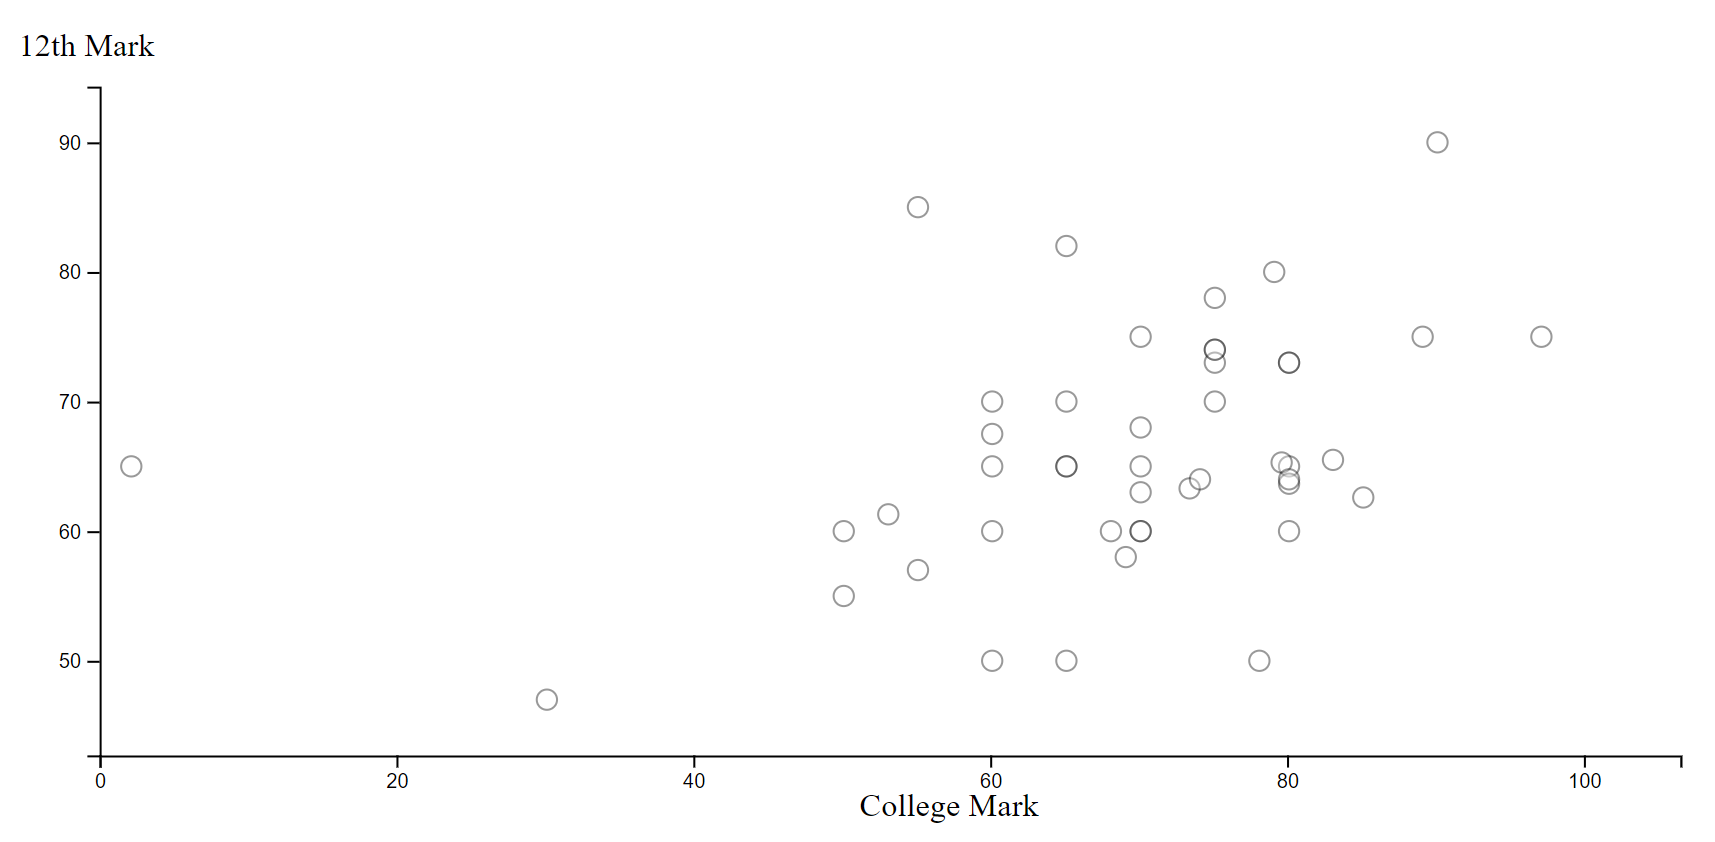
\includegraphics[scale=0.35]{Scatterplot.png}
	\caption{Scatterplot}
	\label{Scatter}
\end{center}
\end{figure}



Warum sich für den Scatterplot entschieden wurde, wurde bereits in \ref{Anforderungen} erläutert, zur genaueren Definition des Scatterplots und wie die \textit{Student Behaviour}-Daten darin dargestellt wurden wird in den folgenden Abschnitten näher darauf eingegangen.
\pagebreak
Der Scatterplot an sich besitzt zwei Achsen, die X-Achse und die Y-Achse. Deren Größe kann entweder manuell bestimmt werden oder hat vier weitere Möglichkeiten gleiche Daten verschieden darzustellen(\cite{Hinneburg2022})\\
\begin{itemize}
\item  X- und Y-Achse haben einen gleich großen Wertebereich
\item Nur die Y-Achse hat einen großen Wertebereich
\item Nur die X-Achse hat einen großen Wertebereich
\item Der Wertebereich in X und Y wird durch die Daten bestimmt
\end{itemize}

Die manuelle Einstellung der Achsen wäre sehr großer Aufwand und auch durchaus ungeeignet, weswegen sich hier für eine dynamische Option entschieden wurde.Die beiden Achsen wurden dem Wertebereich angepasst und können so auch flexibel mit den unterschiedlichen reingeparsten Daten interagieren und sich verändern. In Abbildung \ref{Scatter} enthält in diesem Beispiel die X-Achse als Werte die Daten von College Mark und die Y-Achse die Werte der Daten von 12th Mark.
Zusätzlich zu den dargestellten Achsen und deren Beschriftung enthält ein Scatterplot Punkte, die die verschiedenen zu untersuchenden Individuen und ihre Werte abbilden sollen (in diesem speziellen Fall die Studenten.\\
Aus dem Scatterplot kann also anhand der zwei beschrifteten Achsen und den Punkten auf einen Blick erkannt werden, wie die Notenverteilung bei den unterschiedlich ausgewählten Lernzeiten aussieht.\\

\noindent Wie bereits oben erwähnt können die X- und die Y-Achse dynamisch gewählt werden, genauso wie der \glqq Filter\grqq ,der die Lernzeit auswählt und unter dieser Prämisse die Daten der Noten auswählt

\begin{figure}[h]
\begin{center}
	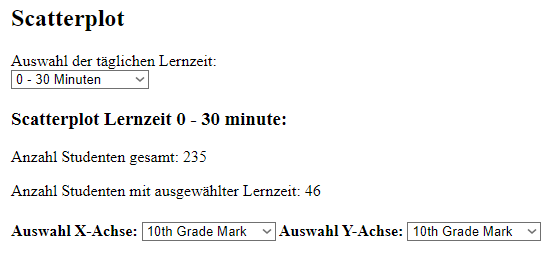
\includegraphics[scale=0.75]{ScatterDrop.png}
	\caption{Ausgewählte Drop-Down-Funktionen und Head}
	\label{ScatterDrop}
\end{center}
\end{figure}

Zu sehen in Abbildung \ref{ScatterDrop} ist, dass die Lernzeit 0-30 Minuten ausgewählt wurde und zusätzlich dazu die bereits erwähnten Achsen. So ist es dem LEser überlassen sich die verschiedenen WErte und differenten Korrelationen der Daten ausgeben zu lassen. Dies stellte eine der Anforderungen an die Visualisierung dar und wurde zusätzlich mit der einfachen Handhabung, gegeben durch die Drop-Downs in die Tat umgesetzt. Es lässt sich so sehr leicht auf einen Blick erkenne, in welchem Notenbereich sich Studenten bewegen, die 0-30 Minuten lernen. Zusätzlich dazu wird die Relation zwischen der Note im College und der Note aus der 12.Klasse abgebildet. \\
Dem Leser werden außerdem zwei zusätzliche Informationen geliefert, einmal wieviele Studenten es insgesamt gibt und außerdem wieviele Studenten von dieser Gesamtanzahl grade ausgewählt sind. Also wieviele Studenten von 235 0-30 Minuten lernen, in dem Fall 46. \\
So kann sich der Leser ein besseres Bild dazu machen, wie sich die Lernzeit grobt verteilt.\\
Außerdem wird dem Betrachter die Hover-Funktion bereitgestellt, dass bedeutet, dass wenn er über die einzelnen Punkte mit der Maus rüber fährt, leuchtet der Punkt grün auf und gibt ihm das Geschlecht mittig über dem Punkt aus.\\

\noindent Eine weiter ähnliche Visualisierungstechnik ist der QQ-Plot, dieser Teil die Datenwerte in verschiede Quantile ein. Hier werden die Verteilunen verglichen, Hinneburg beschreibt es als \glqq Verschiebungen zwischen zwei Verteilungen werden effizient durch Vergleich der Quantile gefunden\grqq \\
\cite{Hinneburg2022}. Da bei der zugrundeliegenden Arbeit allerdings nicht die Quantile veranschaulicht werden sollen, sondern vielmehr die einzelnen Noten der Studenten interessant sind, macht ein Scatterplot deutlich mehr Sinn.

\subsubsection{Parallelplot}
\label{VisZwei}
Die zweite Visualisierung wurde in Form eines Parallelplots dargestellt. Dieser hat, wie bereits in \ref{Anforderungen} gegenüber des Scatterplots den Vorteil, dass hier mehrere Daten auf einmal, sogenannte mehrdimensionale Daten dargestellt werden können.\\ Es können also von einem Studenten unter der Auswahl einer Lernzeitklasse alle Noten auf einmal darstellen. Hierzu werden die verschiedenen Attribute (Noten) vertikal nebeneinander aufgelistet und mithilfe einer Linie verbunden. Diese Linie übernimmt quasi die Aufgabe des Punkts aus dem Scatterplot und veranschaulicht so einzelne Studenten, siehe \ref{Parallel}. Hierbei wurde sich wieder für die Noten 10.Klasse, 12.Klasse \& College Mark zusätzlich zu \textit{Salary expectation} entschieden. So kann die mögliche Korrelation zwischen den einzelnen Noten und der Lernzeit und der Korrelation der einzelnen Noten untereinander gut veranschaulicht werden.\\



\begin{figure}[h]
\begin{center}
	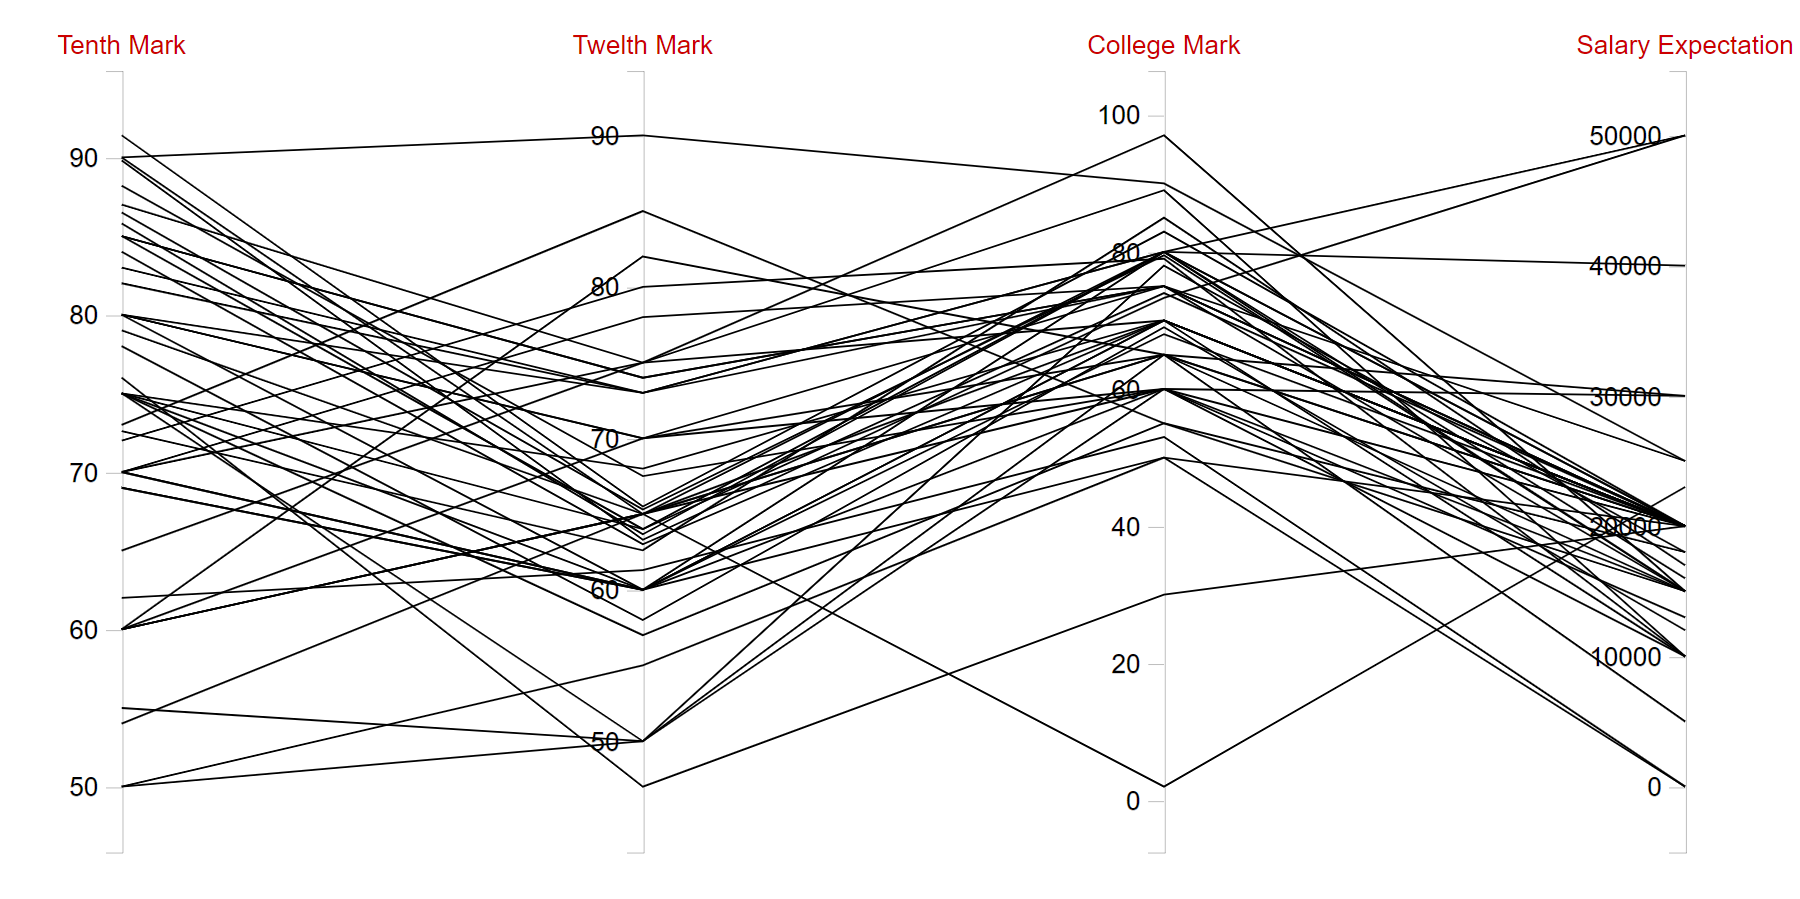
\includegraphics[scale=0.35]{ParallelPlot.png}
	\caption{Parallelplot}
	\label{Parallel}
\end{center}
\end{figure}

\noindent Der Leser erhält außerdem wieder als Kopf über der Visualisierung die Auswahl zwischen den einzelnen Lernzeiten per Drop-Down zu navigieren und erneut die Information, wie viele Studenten es insgesamt und wieviele Studenten es in der jeweils ausgewählten Zeitklasse gibt, siehe Abbildung \ref{ParallelDrop}. \pagebreak

%eventuell erwähnen, dass die Zeitangabe im Header auch dynamisch?

\begin{figure}[h]
\begin{center}
	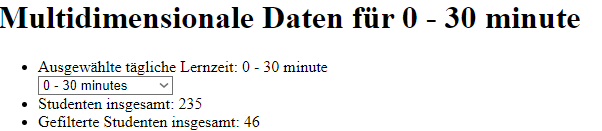
\includegraphics[scale=1]{ParallelDrop.png}
	\caption{Drop-Down Fenster und Head des Parallelplot}
	\label{ParallelDrop}
\end{center}
\end{figure}


\noindent Für den Leser ist so nun, wie in der Zielstellung in \ref{Einleitung} formulierten Anforderung auf einen Blick ersichtlich, wie sich die Verteilung der Noten gestaltet. Sollten sich sehr viele Linien im höheren Segment des Parallelplots ansiedeln, so ist klar, dass in der ausgewählten Lernklasse (in diesem Beispiel 0-30 Minuten)viele Studenten gute Noten in der Schule hatten und immer noch gute Noten im College haben, sowie eine hohe Erwartung an ihr späteres Gehalt haben. Genau das gleiche gilt selbstverständlich für den umgekehrten Fall.\\

\noindent Dem Vorteil der mehrdimensionalen Datendarstellung des Parallelplots steht allerdings die Ünubersichtlichkeit des Gleichnamigen gegenüber. Wenn auch alle Daten auf einmal abgebildet werden können, so leidet darunter die exakte Differenzierung der unterschiedlichen Individuen. Beim Parallelplot ist es also durchaus schwierig die einzelnen Studenten voneinander zu differenzieren. Denn die Linien schneiden sich an den vertikalen Achsen und so ist nicht genau erkennbar, wo welche Linie welches Studenten weiterführt.\\ %daher einführung hover Funktion!


\noindent Genau wie die Parallelen Koordinaten gewährleisten die sternförmigen Koordinaten eine verlustfreie und eindeutige Anordnung der Daten. Im Gegensatz dazu werden die sternförmigen Koordinaten aber nicht parallel nebeneinander angeordnet, sondern es findet eine sternförmige Anordnung der Merkmalsachsen statt \cite{Doerner0304}.\\
Für die Zielsetzung eignet sich der Parallelplot allerdings besser, da es für den Betrachter deutlich leichter ist auf den ersten Blick die Verteilung der Linien einzuordnen. Er kann anhand dieser Verteilung schneller ein Urteil über die Korrelation der Daten fällen, als die bei den sternförmigen Koordinaten der Fall wäre. Hier wäre, wie bereits oben bereits beschrieben, ein gutes mentales Modell und Kenntnisse in Visualisierungsmethoden nötig gewesen, um die Darstellung zu interpretieren; zumindest eine gewisse stärkere Auseinandersetzung mit der Visualisierung an sich.\\

\noindent Eben dieser Fall wollte aber vermieden werden. Es sollte auf den ersten Blick direkt ein ungefähres Urteil über die Daten gefällt werden können und sich dann danach weiter damit auseinandergesetzt werden können. Bei den sternförmigen Koordinaten wäre dies nicht gegeben gewesen. 


\subsubsection{Explizite Baumdarstellung}
\label{VisDrei}
In der dritten und letzten Visualisierung wurde sich für eine explizite Baumdarstellung entschieden. Diese Veranschaulichungsmöglichkeit ist dargestellt als zusammenhängender Graph und die Beziehung zwischen Knoten mit gerichteten Kanten. Außerdem sind alle Knoten von der Wurzel aus erreichbar \cite{Hinneburg2022}.\\
Die auf die Daten angewendete Baumdarstellung ist in Abbildung \ref{Baum} zu sehen.


\begin{figure}[h]
\begin{center}
	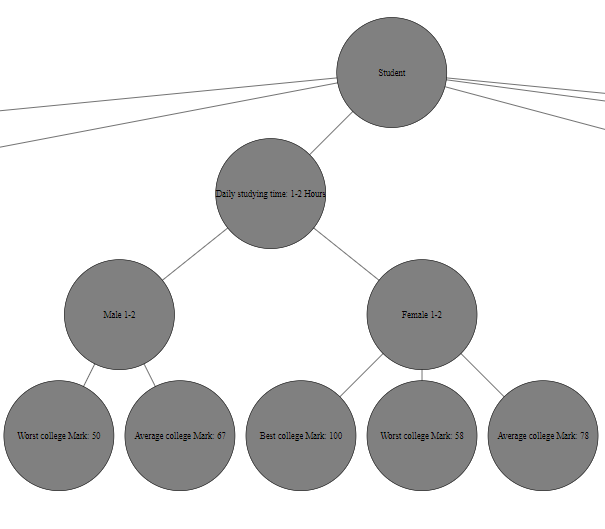
\includegraphics[scale=.75]{BspBaum.png}
	\caption{Explizite Baumdarstellung}
	\label{Baum}
\end{center}
\end{figure}

\noindent Die Wurzel stellt hier der einzelne Student dar. Dieser hat sechs sogenannte Kinder, also Knoten, die mit gerichteten Kanten von ihm wegführen und sie die Beziehung zueinander visuell darstellen. Diese sechs Kinder sind die unterschiedlichen Lernzeiten, die bereits in den vorherigen Visualisierungen immer als Drop-Down zur Verfügung standen.\\
Diese Knoten wiederum haben eine weiter Unterteilung in Männlich und in weiblich, umso erneut zwischen den Geschlechtern Differenzen feststellen zu können.
Die letzten Kinder sind die Noten. Diese wurden diesmal nicht nach Klassen und College unterteilt, sondern nach der besten, schlechtesten und der Durchschnittsnote aus dem College.\\
Der Leser kann so, wie dies bereits in den vorherigen Visualisierungen der Fall war, zuerst die Unterteilung der Studenten nach Lernzeit vornehmen. Und danach kann er nach Geschlecht unterteilen und die jeweiligen Leistungen direkt als String ablesen.\\

Diese Visualisierung hat den Vorteil, dass die exakten Noten inklusive des Durchschnitts dargestellt werden können und so dem Leser direkt als String geliefert werden, es wird also keinerlei Hover-Funktion benötigt. Zudem ist den meisten Lesern die Baumstruktur durchaus aus vielen normalen Lebensbereichen geläufig, wie z.B. der Ordnerstruktur auf dem PC oder der Turnierstruktur bei einer Weltmeisterschaft \cite{Hinneburg2022}.\\
Allerdings bietet die explizite Baumdarstellung auch einige Nachteile, so wird sie sehr schnell unübersichtlich und zu weit verschachtelt, wenn zu viele Knoten dazukommen.\\
Eine andere Möglichkeit wäre daher die implizite Baumdarstellung gewesen, die die grafische Beziehung zwischen Objekten mittels der drei Möglichkeiten

\begin{itemize}
\item Umschließen
\item Überlappen
\item und Berühren
\end{itemize}

\noindent sinnvoll darstellen kann \cite{Hinneburg2022}. Diese haben aber, ähnlich der sternförmigen Koordinaten aus Abschnitt \ref{VisZwei} den Nachteil, dass sie nicht sehr intuitiv für den Leser sind. Der Leser kann bei der ersten Betrachtung, im Gegensatz zur expliziten Baumdarstellung kaum eine Unterteilung der Hierarchie vornehmen. So wird eine der wichtigen Zielstellungen nicht erfüllt. Dieser und der Grund, dass den meisten Menschen die explizite Baumdarstellung weitaus geläufiger ist, wurde sich für letztere Visualisierung entschieden. 






\subsection{Interaktion}
\label{Interaktion}
Der Leser wird zu Beginn der Visualisierung auf die Startseite geführt. Von hier aus hat er mithilfe verschiedener \textit{href} - Buttons die Möglichkeit auf die unterschiedlichen Visualisierungen zu navigieren. Diese Art der Navigation zieht sich über alle Seiten.\\

\noindent Bei der ersten Visualisierung, dem Scatterplot bieten sich dem Nutzer gleich mehrere Interaktionsmöglichkeiten. Zum einen hat er die Auswahl zwischen drei verschiedenen Drop-Down-Funktionen. In der ersten kann er die Lernzeit auswählen. Hierfür stellen sich ihm die Optionen \ref{TimeDrop}. Die beiden anderen Drop-Downs sind gleich aufgebaut und bieten mehrere Möglichkeiten, auf die in \ref{VisEins} bereits näher eingegangen wurde.

\begin{figure}[h]
\begin{center}
	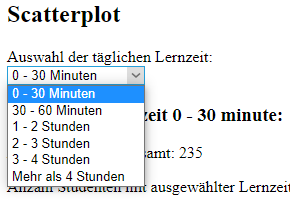
\includegraphics[scale=.75]{ScatterZeitDrop.png}
	\caption{Drop-Down Funktion der Lernzeit}
	\label{TimeDrop}
\end{center}
\end{figure}

\noindent Eine weiter Interaktionsmöglichkeit beim Scatterplot stellt die \textit{Hover} - Funktion dar,die dem Nutzer zusätzliche Informationen liefert. Wenn der Nutzer über die einzelnen punkte \textit{hovert}, so leuchtet der ausgewählte Punkt grün auf und liefert als \glqq Ausgabe\grqq mittig darüber das Geschlecht und die präferierte Lernzeit, genauer ist die in Abbildung \ref{ScatterAnw} zu sehen.

\begin{figure}[h]
\begin{center}
	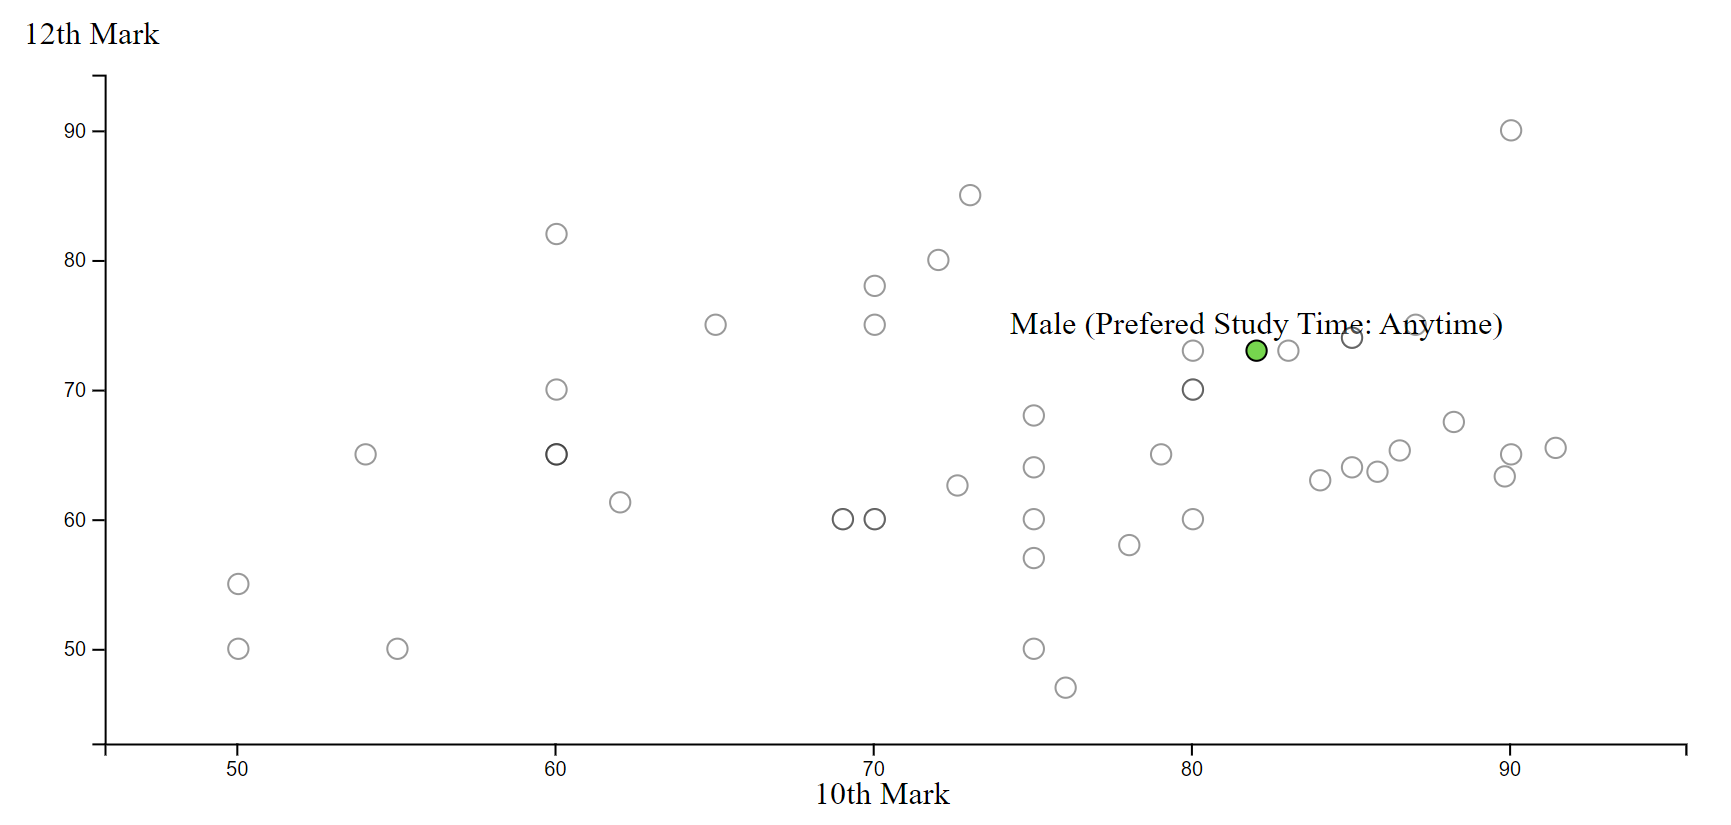
\includegraphics[scale=.25]{ScatterAnw.png}
	\caption{Scatterplot mit Hover-Funktion}
	\label{ScatterAnw}
\end{center}
\end{figure}

\noindent Wie beim Scatterplot hat der Nutzer beim Parallelplot die Auswahlmöglichkeit der Drop-Down-Funktion für die Lernzeit, siehe Abbildung \ref{TimeDrop}.\\
Zusätzlich dazu wird hier die Möglichkeit gegeben, die Anordnung der Achsen beliebig anzuordnen. Dies wird diesmal in Form von Button abgebildet um eine größere Breite an Interaktionsmöglichkeiten abzudecken, siehe Abbildung \ref{Buttons}. Hier gibt es für jede Achse dieselbe Auseahl an Variablen. Es wäre in der Theorie also auch möglich für jeden Achse denselben Wert festzulegen.

\begin{figure}[h]
\begin{center}
	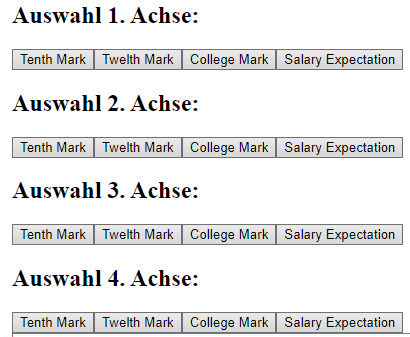
\includegraphics[scale=.5]{WahlAchse.png}
	\caption{Parallelplot mit Button für die Auswahl der Achsen}
	\label{Buttons}
\end{center}
\end{figure}

Bei dem Baumdiagramm ist die Reihenfolge und Hierarchie bereits durch die Beschaffenheit des Diagramms an sich fest. Hier kann allerdings zusätzlich dazu durch die Eingabe der Breite, Höhe und des Radius die Visualisierung des Baums verändert werdend. Der Nutzer hat also keine vorher festgelegte Auswahl, sondern kann fast komplett frei entscheiden, was er in das \textit{input} - Feld schreibt. Die einzige Bedingung, die hier gilt ist, dass es sich um einen Float handeln muss.



\section{Implementierung}

Die nächsten Abschnitte behandeln die Implementierung des Codes. Für die Implementierung wurde sich an den Übungen orientiert und dieser Code dann übernommen und angepasst. Für \ref{ScatterParallel} an Übung 1 und  Übung 6 und für\ref{ImplBaum} an Übung 7.\\

\subsection{Scatterplot und Parallelplot}
\label{ScatterParallel}

\noindent Jede einzelne Datei besteht grundlegend aus einem \textit{main}, welches die Funktionen \textit{init}, \textit{update} \textit{subsriptions} und \textit{view}, siehe Abbildung \ref{Main}.
Der erste Schritt war die Daten zu laden und zu Decoden. Dabei wurde sich wieder am Code der Übung 7 orientiert. Die Daten wurden aus der \textit{Student\_Behaviour.csv}-Datei geladen, die im Github abgelegt war. Das Laden der Daten geschah über die eben erwähnte \textit{init}-Funktion, bei der mtihilfe eines \textit{Http.get}-Befehls der Link aus dem eigenen Github geladen wurde. Auf die anderen funktionen wird später genauer und individuell eingegangen.







\begin{figure}[h]
\begin{center}
	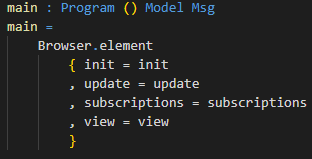
\includegraphics[scale=.75]{Main.png}
	\caption{Main}
	\label{Main}
\end{center}
\end{figure}


\noindent Nachdem die Laden über die \textit{init}-Funktion geladen wurden, müssen sie nun dekodiert werden.
Zuerst mussten die verschiedenen Module dafür geladen und importiert werden, in diesem Fall \glqq Csv\grqq und \glqq Csv.Decode\grqq. %möglicherweise Einfügen Abbildung oder ähnliches und dann Aufführung weiter unten?
Mithilfe dieser Module konnte die Funktion zum codieren der Daten geschrieben werden, dieser Code ist zu sehen in Abbildung \ref{Decode}.\\


\begin{figure}[h]
\begin{center}
	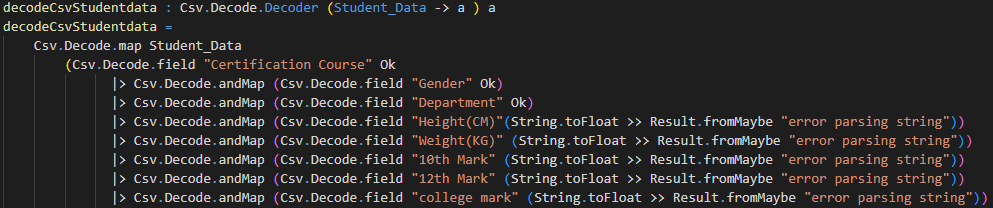
\includegraphics[scale=.5]{decode.png}
	\caption{Ausschnitt der Decode-Funktion}
	\label{Decode}
\end{center}
\end{figure}

\noindent Hier werden die einzelnen Daten als String reingeparst und falls sie auch ein String in der weiteren Verarbeitung sein sollen als \glqq Ok\grqq markiert. Falls sie umgeformt werden sollen, wird dies mit der Anweisung \glqq String.to\grqq und danach der gewünschte Datentyp, z.B. Float erreicht. In einem Beispiel im Datensatz wäre das beispielsweise bei \textit{10th Mark} der Fall. Damit in elm aber weiter damit als Float gearbeitet werden kann, muss dieser Datentyp nochmal in einem \textit{type} definiert werden. Die Daten wurden also im \textit{type} \textit{Student\_Data} nochmals definiert um mit ihnen später weiterarbeiten zu können. Hier mussten sie als genau der Datentyp definiert werden, als der sie auch vorher decoded wurden. Sonst warf es eine Fehlermeldung aus. Die \textit{type}-Definition sah dann wie in Abbildung \ref{Type}. Das Decodieren war zu Anfang eine sehr mühselige Arbeit und nahm einiges an Zeit in Anspruch, da hier alle Strings genauso geschrieben werden mussten, wie in der Csv-Datei. Da es auch ein paar Rechtschreibfehler gab (z.B. \glqq social medai\grqq statt \glqq social media\grqq und teilweise Leerzeichen hinter den Strings standen (beispielsweise bei \glqq stress level\grqq war dies anfänglich etwas frustrierend. 



\begin{figure}[h]
\begin{center}
	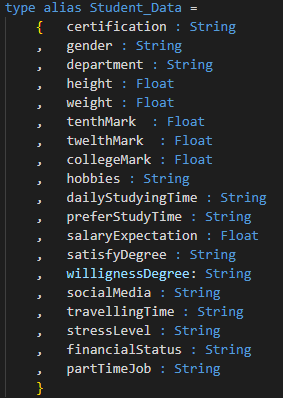
\includegraphics[scale=.75]{typeDef.png}
	\caption{Ausschnitt der \textit{type} - Definition Student\_Data}
	\label{Type}
\end{center}
\end{figure}

\noindent Der grundlegende Aufbau des Elm-Programms setzt sich aus vier Dateien zusammen, der \textit{Scatterplot\.elm}, \textit{Baumvisualisierung\.elm}, \textit{ParallelPlot\.elm} und  \textit{Main\.elm}. Jede Datei steht für die jeweilige Visualisierung, während die \textit{Main\.elm}-Datei die Startseite der Website darstellt.\\

\noindent Der Aufbau der kompletten Visualisierung stellte ein weiteres größeres Problem dar. Die Verknüpfung der einzelnen \textit{case of} - Fälle ließ sich von mir nicht ohne jegliche Fehlermeldung lösen. Daher musste auf eine andere Art der Technik zurückgegriffen werden. Anstatt alles auf eine Seite zu laden, wurde hier mit einer \textit{Seitennavigationsleiste} gearbeitet %Bild einfügen, wenn Leiste steht.
So kann zwischen den einzelnen Visualisierungen navigiert werden, siehe Abbildung \\%\ref{Navigation}.

\noindent Zusätzlich zur \textit{type} - Definition Student\_Data wurden bei allen Visualisierungen ein \textit{type Msg} definiert. In diesem wurden die verschiedenen Aktionen festgelegt, die dem Leser bei \ref{Interaktion} zu Verfügung stehen , also die Lernzeit (\textit{ChangeStudTime}), oder die Daten für die Achsen (\textit{ChooseStudent1}, \textit{ChooseStudent2}) zu bestimmen. Zu sehen in Abbildung \ref{MsgScatter}. 

\begin{figure}
    \subfigure[\textit{type} - Definition \textit{Msg}]{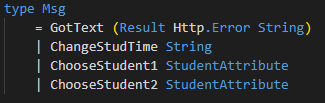
\includegraphics[width=0.49\textwidth]{typeMsg.png}}
    \subfigure[\textit{type} - Definition \textit{StudentAttribute}]{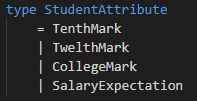
\includegraphics[width=0.49\textwidth]					{typeStudentAttribute.png}}
\caption{\textit{type} - Definition im Beispiel Scatterplot}
\label{MsgScatter}
\end{figure}

\noindent Bei dem \textit{type StudentAttribute} werden die Daten festgelegt, die später an den Achsen des Scatterplots abgebildet werden und dynamisch ausgewählt werden könne, in diesem Fall also die Noten aus der 10., 12. Klasse, aus dem College und die Erwartungen an das spätere Gehalt.\\

\noindent Beim Parallelplot verhält sich diese Funktionalität ähnlich, es mussten nur zwei weitere Funktionen hinzugefügt werden und diese wurden dann auch direkt in die \textit{type Msg} eingebettet.
Bei beiden Plots wurden zudem Punkte definiert, beim Scatterplot eine \textit{type Point} und beim Parallelplot eine \textit{type MultiDimPoint}.\\

\noindent Weiterhin wurden bei beiden die \textit{Html} Drop-Down Funktion als eingefügt, damit der Leser auf der Website auswählen kann. Die drei Funktionalitäten, Auswahl X-, Y-Achse und LErnzeitasuwahl hatten alle denselben Aufbau. Sie bekamen den Value aus dem Datensatz gegeben und hatten ein \glqq Html.text\grqq Feld, welches dem Nutzer angezeigt wird. Mit \glqq Html.select\grqq konnte der Nutzer nun zwischen den vorher festgelegten Feldern auswählen.\\

\noindent Diese Auswahl wurde in der \textit{update} - Funktion verarbeitet, siehe Abbildung \ref{updateScatter}. Diese interagiert mit der \textit{type Msg} und arbeitet mit der \textit{case of}. Bei \glqq GotText\grqq werden (in den folgenden Beispielen wird immer davon ausgegangen, dass es zu keiner Fehlermeldung kommt) die Daten geladen und ein \textit{Default} - Wert festgelegt, in diesem Fall liegt also die Lernzeit beim erfolgreichen Laden der Daten bei 0-30 Minuten und die Punkte auf der X-Achse als Noten der 10. Klasse und Y-Achse bei Noten der 12.Klasse.\\
Falls der Nutzer die Zeit ändert, also die Funktion \glqq ChangeStudTime\grqq aufruft, werden die Daten dahingehend geändert, dass nun, bei gleichbleibenden Achsen (also Noten 10. und 12.Klasse) die Werte sich auf den gewünschten neuen Wert anpassen. Also würde z.B. die Lernzeit auf 1-2 Stunden angehoben werden, wird dies entsprechend angepasst. Gleiches gilt bei Änderung der Achsen. Hier tritt der Fall \glqq ChooseStudent1\grqq oder \glqq ChooseStudent2\grqq ein, je nachdem welche Achse geändert wird.
Sollte es hier bei einem der Schritte zu einem Fehler kommen, wird die \glqq Error-Funktion\grqq durchgeführt.\\

\noindent Bei beiden Plots wurden die Daten zudem noch gefiltert, welche dann in der \textit{view} - Funktion aufgerufen wurden. Diese \textit{view} - Funktion sah auch bei beiden ähnlich aus, sie handelte zuerst die Optionen des \textit{Failure} und \textit{Loading} um bei einem \textit{Success} die Daten und den Plot darzustellen. Hier wurden erst die verschiedenen Werte im \textit{let} - Teil definiert um sie danach im \textit{in} - Teil mit dem Plot an sich darstellen zu können. Im \textit{in} - Teil wurden außerdem die verschiedenen \textit{Html} - Attributen und \textit{hrefs} aufgelistet.\\



\begin{figure}[h]
\begin{center}
	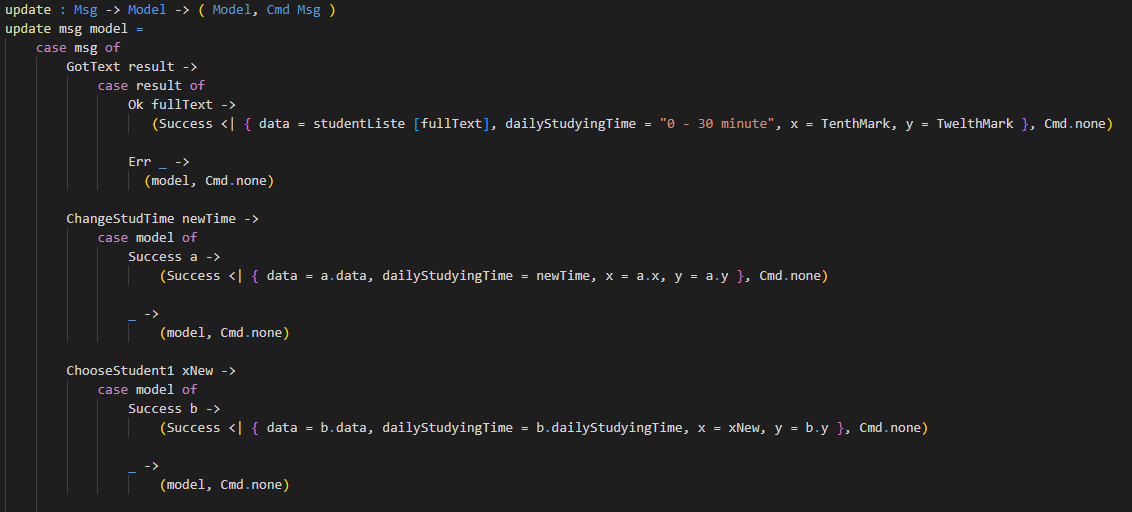
\includegraphics[scale=.5]{updateScatter.png}
	\caption{Ausschnitt der update-Funktion aus dem Scatterplot}
	\label{updateScatter}
\end{center}
\end{figure}






\noindent Beim Scatterplot, welcher als erster visualisiert wurde, wurde die ungefähre Struktur aus den ersten Übungen übernommen. Hier mussten nachdem die Eckpunkte des Scatterplots aufgestellt worden waren, die Punkte und \textit{Maybe Points} erstellt werden. Zusätzlich dazu die Achsenbeschriftung und die oben bereits erwähnten \textit{update} und \textit{view} - Funktionen integriert werden. Danach erfolgte noch weitere Personalisierungen der Visualisierungen um sich die gewollten Werte anzeigen zu lassen.\\

\noindent Ähnlich wurde beim Parallelplot vorgegangen, wobei der \textit{type Msg} hierfür noch um zwei weitere Variablen erweitert wurde, damit alle Möglichkeiten für die Achsen abgedeckt wurden. Bei der Erstellung dieser Visualisierung wurde sich an der Übung sechs orientiert. Dadurch, dass diese auch bereits die Option des Daten-Laden behandest, ging dies deutlich schneller als die Erstellung des Scatterplots. Auch hier wurde wieder, wie beim Scatterplot mit der Hover-Funktion gearbeitet, um die einzelnen zu betrachtenden Datenwerte besser hervorheben zu können.


\subsection{Explizite Baumdarstellung}
\label{ImplBaum}

\noindent Für die Visualisierung der expliziten Baumdarstellung wurde sich an Übung 7 orientiert. Die Daten wurden 


\noindent Der \textit{type Msg} ähnelt wieder dem der Plots s. Abbildung \ref{MsgScatter}, mit den veschiedenen dynamischen Möglichkeiten, die dem Nutzer gegeben werden um mit der Webseite zu interagieren. Die Daten wurden wieder über die \textit{init} - Funktion geladen. Allerdings wurden sie diesmal nicht aus einer Csv-Datei geladen, sondern aus einer \textit{json}. Wie bereits in \ref{Datenvorverarbeitung} erwähnt, wurde diese hierfür manuell aus der Csv-Datei erstellt, damit mit dieser gearbeitet werden konnte. Im Gegensatz zu den vorherigen Plots wurde bei der Baumvisualisierung eine andere Form der Datendecodierung gewählt, die aus der Übung 7 übernommen wurde, siehe Abbildung \ref{treeDecode}.


\begin{figure}[h]
\begin{center}
	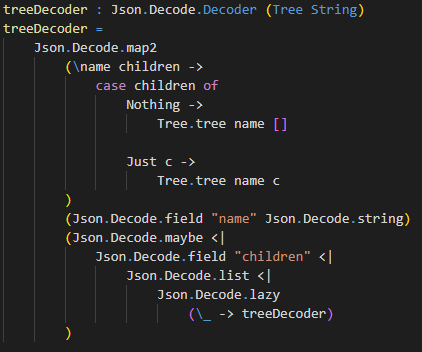
\includegraphics[scale=.75]{treeDecode.png}
	\caption{Decode Funktion der Baumvisualisierung}
	\label{treeDecode}
\end{center}
\end{figure}


\noindent Die Interaktionsmöglichkeiten s. mehr dazu in \ref{Interaktion} sind ähnlich aufgebaut wie bei Scatterplot und Parallelplot. In der \textit{update} - Funktion werden die verschiedenen Messages angegeben, in denen die Optionen abgedeckt werden vgl. . \ref{updateScatter}, die dem Nutzer vorliegen. Also die Höhe, Weite, etc. des Baumdiagramms zu ändern. Wie in den beiden Plots die Punkte \glqq gezeichnet\grqq wurden, so werden hier mit den Funktionen \textit{Knoten} und \textit{Kanten} die Knoten und Kanten \glqq gezeichnet\grqq . Die Kanten verbinden die einzelnen Knoten miteinander, um so das explizite Baumdiagramm darstellen zu können.\\

\noindent Am schwierigsten gestaltete sich bei dieser Implementierung das Laden der Daten. Genauer gesagt das Umstrukturieren der Csv-Datei in eine \textit{json}. Hierbei wurde anfangs versucht dies mit einer \textit{python} - Anwendung umzuschreiben. Dieser Ansatz funktionierte leider nicht, da die Funktion keine genestete Datei als Ergebnis ausgab und es somit nicht für die Baumdarstellung genutzt werden konnte. \\
Nach mehrmaligem Rumprobieren wurde die Datei daher manuell erstellt. Dies führte allerdings zum nächsten Problem: Bei der Darstellung der verschiedenen Noten kam es häufig zu Dopplungen bei den \textit{children}, da sich beispielsweise die Noten der besten Frau mit Lernzeit 0-30 Minuten mit der besten Frau der Lernzeit 30-60 Minuten deckten. % Hierfür wurde xy.
%ergänzen



\section{Anwendungsfälle}

.... Da nicht einzelne Personen, sondern Muster im großen ganzen erkannt werden sollen, stellt es sich etwas schwieriger dar, dieses als einzelnes Bild in der Hausarbeit darzustellen. Vielmehr sollte der Leser dies in den Visualisierungen selber ausprobieren.

\begin{itemize}
\item Informationsbeschaffung Elternteil des Notenverlaufs bei verändernder Lernzeit
\item Verlauf und Zusammenhang der Noten mit sich ändernder Lernzeit
\item Korrelation Notendurchschnitt mit Geschlecht und Lernzeit
\item Der Wertebereich in X und Y wird durch die Daten bestimmt
\end{itemize}

Präsentieren sie für jede der drei Visualisierungen einen sinnvollen Anwendungsfall in dem ein bestimmter Fakt, ein Muster oder die Abwesenheit eines Musters visuell festgestellt wird. Begründen sie warum dieser Anwendungsfall wichtig für die Zielgruppe der Anwenderinnen ist. Diskutieren sie weiterhin, ob die oben beschriebene Information auch mit anderen Visualisierungstechniken hätte gefunden werden können. Falls dies möglich wäre, vergleichen sie die den Aufwand und die Schwierigkeiten ihres Ansatzes und der Alternativen. 


\subsection{Anwendung Visualisierung Eins}
\label{AnwEins}
Ein Anwendungsfall mit dem Scatterplot wäre ein Elternteil, dass sehen will, wie sich die Noten der Studenten über die Jahre hinweg unter dem Einfluss der Lernzeit ansehen, um so eventuell Rückschlüsse auf das eigene Kind und deren mögliche Entwicklung zu ziehen. Dem Elternteil soll also die Gesamtverteilung der Noten nach einer eigen vorgenommenen Filterung zur Verfügung gestellt werden, sodass sie sich einen guten, möglichst unvoreingenommenen Überblick verschaffen kann. Der Scatterplot soll die Daten fast schon \textit{plain} darstellen, sodass dem Benutzer keinerlei Dinge suggeriert werden.\\

\noindent Dies ist, wie in Abbildug \ref{ScatterAnw} zu sehen ist sehr gut gelungen. Der Nutzer bekommt eine sehr einfache Visualisierung vorgestellt, auf denen er einzig die Achsen und die dargestellten Einzeldaten einsehen kann. Beim Fahren mit der Maus über die einzelnen Punkte erhält der Leser allerdings kleine weiter Informationen, wie das Geschlecht und die Zeit, in welcher die Studenten am liebsten lernen. Im Gegensatz zum Parallelplot in \ref{AnwZwei} sind dies wenige und Informationen. So soll weiterhin gewahrt werden, dass der Leser einen allgemeineren Überblick behält.


\noindent Mithilfe der in \ref{Interaktion} erläuterten \textit{Hover} - Funktion lässt sich hier außerdem weitere Informationen über den Einfluss der Lernzeit generieren. So wird nicht nur die Dauer beachtet, sondern zusätzlich noch die Uhrzeit am Tag.


\subsection{Anwendung Visualisierung Zwei}
\label{AnwZwei}
Im zweiten Beispiel wird eine Visualisierung anhand des Parallelplots angewandt. Hier wird der Notenverlauf in Abhängigkeit der Variable Lernzeit und der am Ende verbundenen Gehaltserwartung untersucht. Es sollte also erkennbar sein, dass Studenten die viel Lernen gute Noten und auch eine höhere Gehaltsvorstellung haben, als wenig lernende Studenten, die eher schlechte Noten und dahingehend auch mit schlechterem Gehalt rechnen sollten.\\

\noindent Das dies allerdings nicht immer der Fall ist zeigt sich vor allem deutlich bei der Lernzeit \glqq Mehr als 4 Stunden \grqq . Hier hat eine Studentin also die höchstmöglich auswählbare Lernzeit angegeben und war zwar in der 10. Klasse mit der Note \textit{80} und der 12. Klasse mit \textit{70} zwar noch relativ gut, ging im aber deutlich nach unten. Hier erreichte sie nur die Note \textit{12}. Sie hat also trotz sehr hohem Lernaufwand im College schlechte Noten und gibt trotzdessen den in dieser Rubrik höchsten Wert in der Gehaltserwartung an, mit \textit{30000}.\\

\noindent Dies spiegelt also in keinster Weise die im vorhinein getroffenen Erwartungen wieder, dass die vier Variablen bei allen in einem Zusammenhang stehen.\\
Natürlich lässt sich nicht von einem Individuum auf alle schließen und könnte als Ausreißer dargestellt werden, dennoch spricht es gegen die aufgestellte These.\\

\noindent Viele Gegenbeispiele lassen sich zudem bei der Lernzeit \glqq 0-30 Minuten herausfiltern\grqq . Trotz der relativ niedrigen Lernzeit gibt es viele Studenten, die gute bis sehr gute Noten über die Klassen und das College hinweg haben. Zwei dieser Beispiele sind deutlich in Abbildung \ref{BspPar} zu sehen.


\begin{figure}
\begin{center}
    \subfigure[]{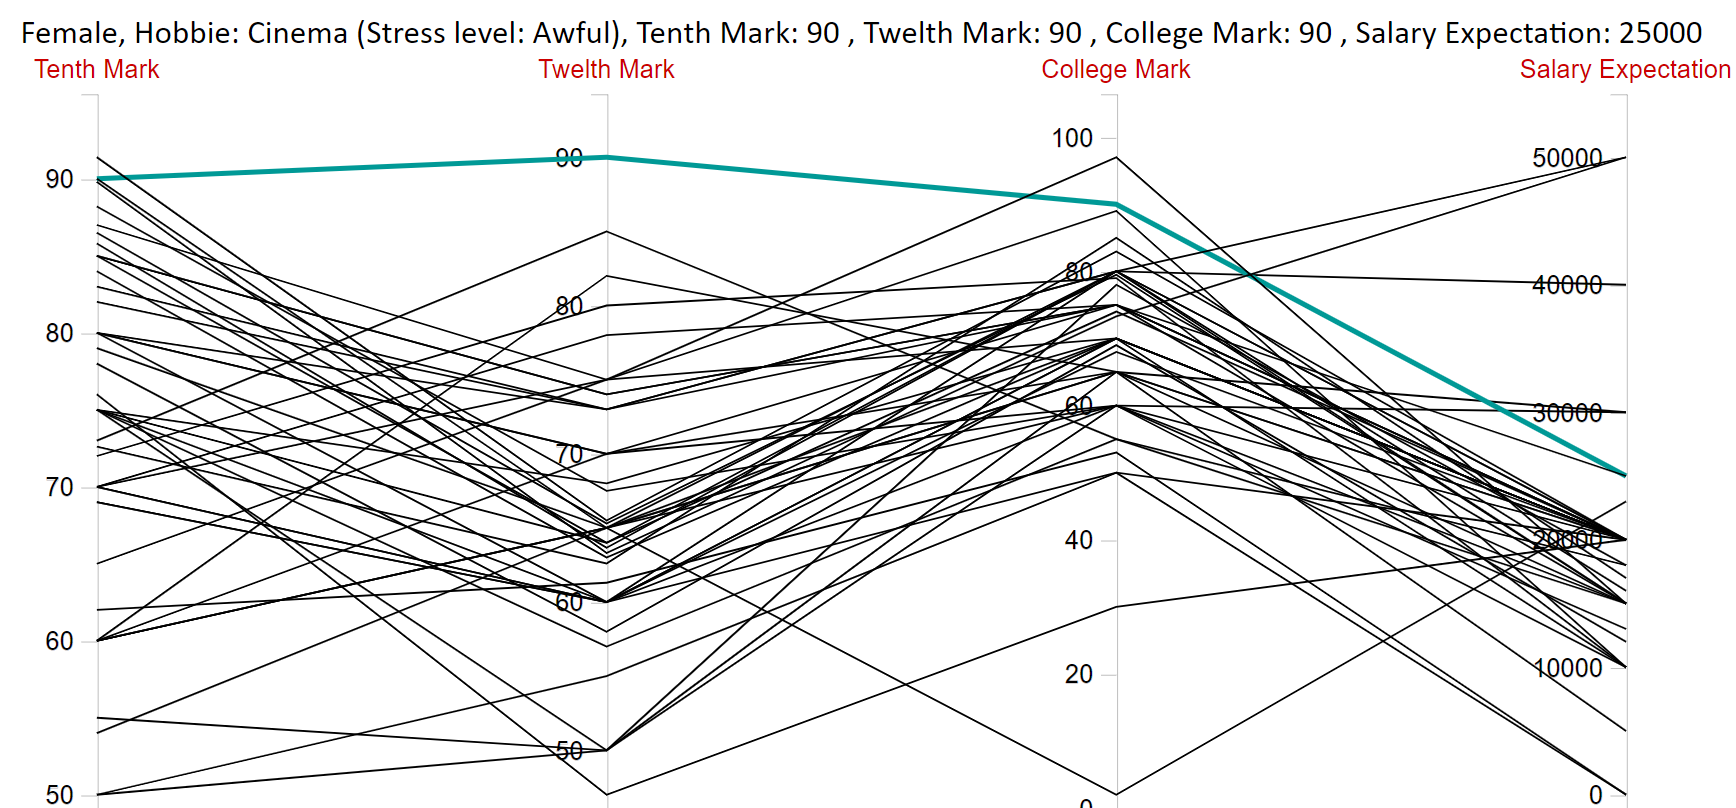
\includegraphics[width=.75\textwidth]{BspPar1.png}}
    \subfigure[]{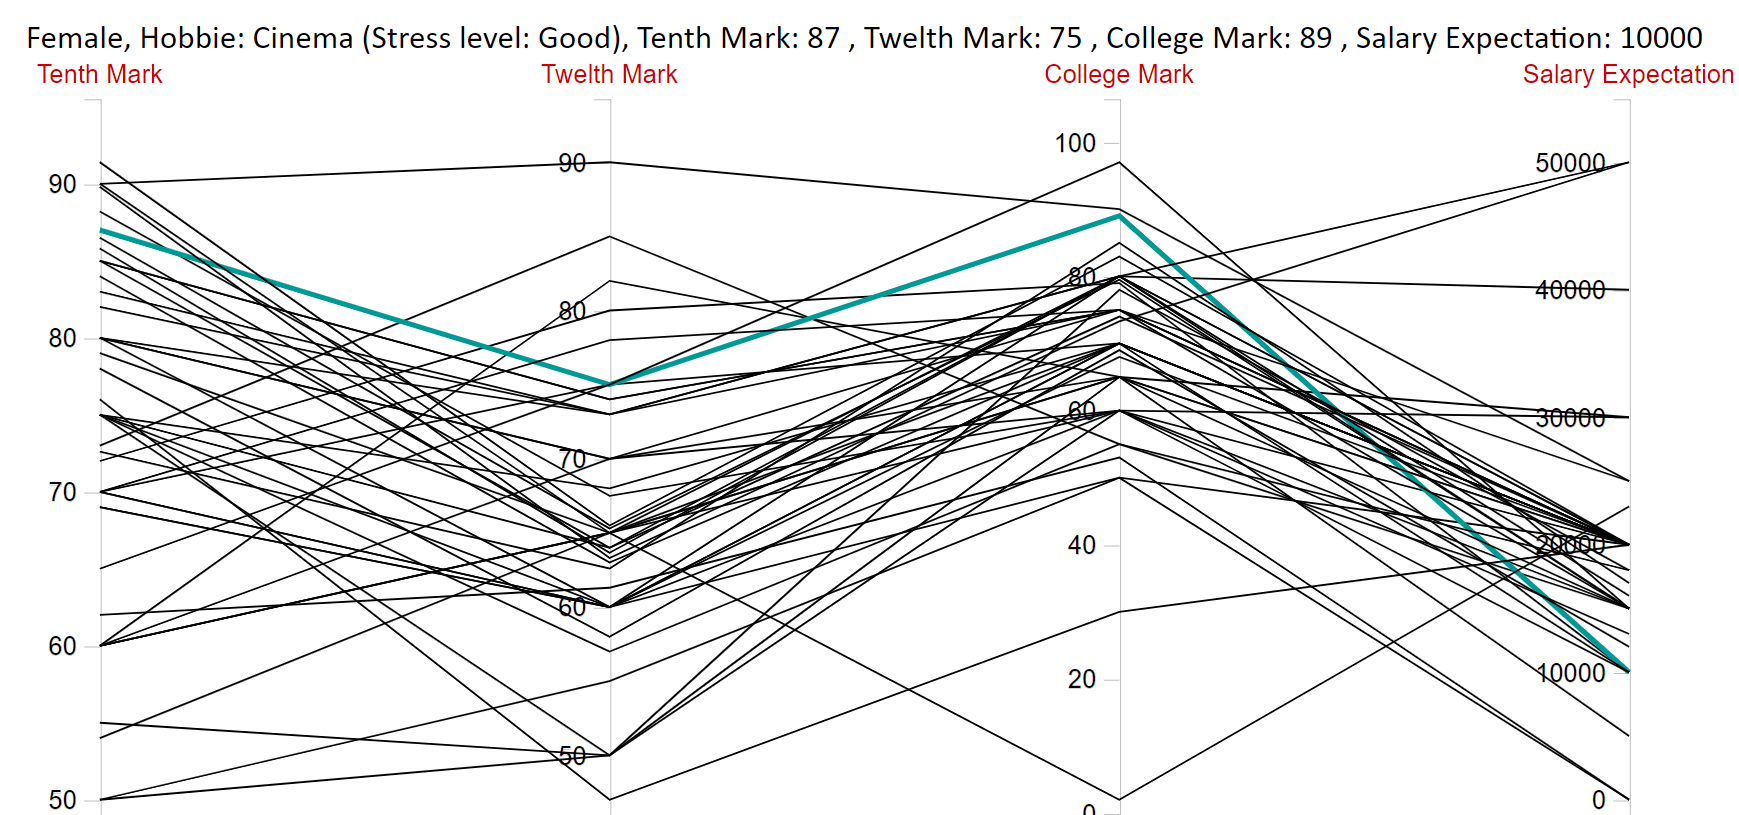
\includegraphics[width=.75\textwidth]					{BspPar2.png}}
\caption{Zwei Beispiele Parallelplot - Lernzeit: 0 - 30 Minuten}
\label{BspPar}
\end{center}
\end{figure}



\subsection{Anwendung Visualisierung Drei}
\label{AnwDrei}

Da bei der Baumvisualisierung erst im Geschlecht und dann in die verschiedenen Lernzeiten unterteilt wird und als letztes \glqq Kind\grqq der Durchschnitt gezeigt wird, soll geschaut werden, inwieweit sich der Durchschnitt bei steigendern Lernzeit verändert. Auch die Differenzen zwischen den Geschlechtern soll hier beachtet werden.Dies ist in der gezeigten Abbildung \ref{WoMenTree} nocheinmal bildlich visualisiert worden.


\begin{figure}
\begin{center}
    \subfigure[Baumdiagramm Männer]{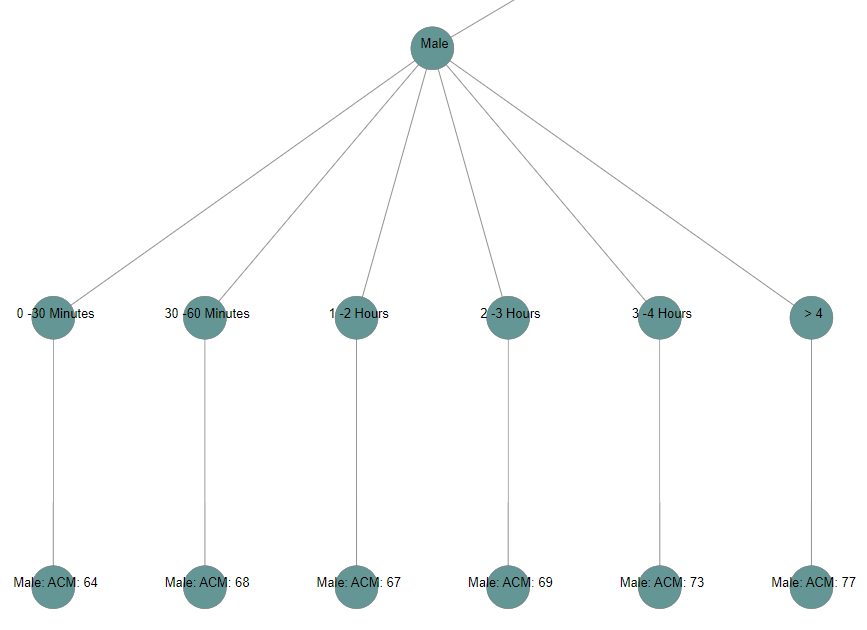
\includegraphics[width=.75\textwidth]{MenTree.png}}
    \subfigure[Baumdiagramm Frauen]{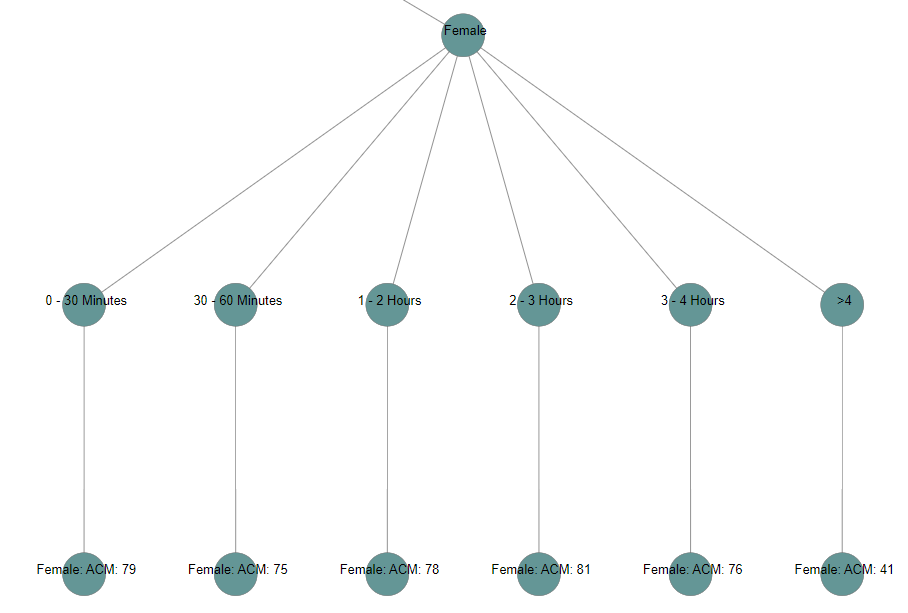
\includegraphics[width=.75\textwidth]					{WomenTree.png}}
\caption{Gegenüberstellung des Notendurchschnitts der Lernzeit bei Männern und Frauen}
\label{WoMenTree}
\end{center}
\end{figure}

\noindent Bei den Männern ist eine durchaus positive Korrelation zwischen der Lernzeit und dem Notendurchschnitt zu erkennen, vor allem wenn die beiden Extrema verglichen werden. Bei der geringsten Lernzeit liegt der Durchschnitt bei 64, wohingegen er bei der höchsten Lernzeit bei 77 liegt. Es ist also ein starker Anstieg von 13 Notenpunkten im Durchschnitt zu erkennen. Zudem ist eine fast permanente Steigung über alle Lernzeiten hinweg zu erkennen. Nur einmal sinkt der Wert anstatt zu steigen und zwar von 68 auf 67. Danach steigt der Wert jedoch  wieder zweimal an.\\
\noindent Bei den Männer lässt sich anhand der vorliegenden Grafik also die Aussage treffen, dass die Lernzeit und der Notendurchschnitt positiv miteinander korrelieren.\\

\noindent Bei den Frauen ist dahingehend leider keine ähnliche Aussage zu treffen. Vor allem der Ausreißer bei der höchsten Lernzeit von über 4 Stunden zieht den Durchschnitt sehr nach unten. Dies ist aber wahrscheinlich auf die geringen Anzahl der Frauen in diesem Segment zurückzuführen. Zudem ist hier keine stetige Steigung der Werte zu erkennen. \pagebreak




\section{Verwandte Arbeiten}
In der ersten Arbeit von xyz wurde \glqq PerformanceVis\grqq entwickelt, ein visuelles analytisches Werkzeug, mit dessen Hilfe die Leistung und Zulassungsfähikeit der Studenten geprüft werden soll. Hierfür wurde ein Einführungskurs in Chemie der Universitätsweit angeboten wird, mit knapp 1000 Studenten untersucht. Dort wurden in einer Onlinelernplattform Dinge getrackt, wie z.B. Die Häufigkeit der Logins, die Benutzung verschiedener Hilfsmittel und \glqq PerformanceVis\grqq hat sich dabei hauptsächlich auf die Lernspuren der Schüler fokussiert.\\

\noindent Wie in der hier beschriebenen Arbeit und der angefertigten Visualisierungen arbeitet auch \cite{Deng19} mit mehreren Parallelplots, wovon einer in Abbildung dargestellt ist. Hierbei wurden zwei Zielgruppen miteinander verglichen, gekennzeichnet mit den beiden unterschiedlichen Farben. Während die blau gefärbten \textit{polylines} Schüler darstellen, die ein \textit{C} sowohl im dritten als auch dem letzten Examen darstellen, repräsentieren die orangen gefärbten \textit{polylines} Schüler, die im dritten Examen ein \textit{C}, im finalen Examen aber ein \textit{A} hatten. Es ist also deutlich erkennbar, dass die Schüler die zu Beginn in den ersten beiden Examen gut waren sich deutlich besser \glqq erholten\grqq von einem \textit{C}, als Schüler, die davor bereits schlechte Noten hatten.\\






\begin{figure}[h]
\begin{center}
	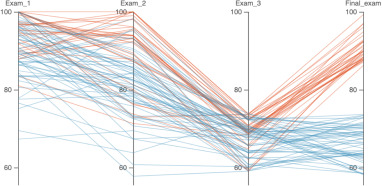
\includegraphics[scale=1.3]{ParallelQuelle1.jpg}
	\caption{Parallelplot mit den unterschiedlichen \glqq Exams\grqq}
	\label{Quelle1}
\end{center}
\end{figure}


\noindent Für das \textit{tool} \glqq PerformanceVis\grqq und zum besseren Verständnis der \glqq student performance [fluctuation] throughout the course, we should display the grade distributions for each exam.\grqq  \cite{Deng19}. Es wurde also Wert darauf gelegt diese Fluktuation mithilfe der Notenverteilung in einem Parallelplot darzustellen, genauso wie es auch in dieser Arbeit der Fall war. Bei dieser Arbeit und vor allem bei dieser Visualisierung ist die Schlussfolgerung, dass die Noten sich untereinander beeinflussen. Bei der eigenen Arbeit konnten wir nicht zu dem gleichen Schluss kommen. Allerdings ist dies wahrscheinlich eher auf die Diskrepanz in der Stichprobengröße zurückzuführen, da in \cite{Deng19} diese fast viermal so groß ist (~1000 zu ~250).\\
Was sich allerdings ähnelt ist die Art der Visualisierungen. In \cite{Deng19} wurde sich nicht nur auch für den Parallelplot, sonder außerdem auch für ein Baumdiagramm entschieden.\\


\noindent Das Paper von \cite{Xu14} behandelt als eins der wenigen wissenschaftlich auffindbaren Paper im Bereich Informationsvisualisierung den Zusammenhang \textit{Student Behaviour} und diesen Einfluss auf das Abschneiden der Studenten. Dafür werden die nötigen Charakteristiken der studentischen Teilnehmer an den MOOCs (Massive Open Online Courses) visuell beschrieben. Von \cite{Xu14} wird zitiert, dass weder Alter noch Geschlecht Einfluss auf den höchsten Abschluss haben. Zu ähnlichen Ergebnissen kam diese Arbeit, als sich keine signifikanten Unterschiede zwischen Männern und Frauen bei dem \textit{Grade average} offenbarte.\\

\noindent In diesem Paper wurde eine etwas andere Art der Visualisierung gewählt \ref{Quelle2} und auch ein etwas anderer Ansatz. Xu geht hier nicht so sehr auf den Einflussfaktor Lernzeit ein, sondern vielmehr auf das stetige Mitarbeiten in einem Kurs mit Einfluss auf die Noten. Das stetige Mitarbeiten wird hier im Sinne von \glqq quiz submissions\grqq dargestellt.\\



\begin{figure}[h]
\begin{center}
	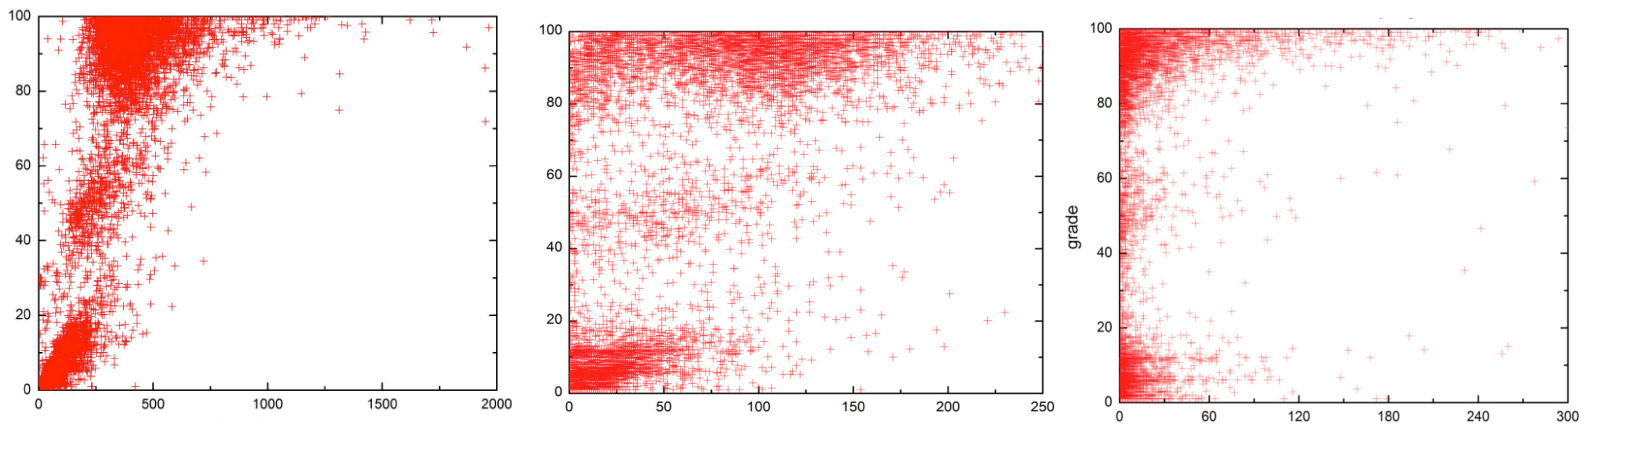
\includegraphics[scale=.3]{Quelle2.png}
	\caption{Plots von \glqq Grades\grqq against \glqq quiz submissions\grqq}
	\label{Quelle2}
\end{center}
\end{figure}

\noindent Weiterhin beschreibt \cite{Xu14}\: \glqq [...] there are multiple ways to be
successful in a course, and it is perhaps not necessary to do
everything – at least, not for everyone\grqq .\\
Er stellt hier also die These auf, dass es nicht unbedingt den einen einzelnen Einflussfaktor auf die Note und Erfolgsquote in einem Kurs gibt. Wie auch wir bereits in \ref{Einleitung} ähnlich beschrieben haben gibt es deutlich mehr, viele davon lassen sich nicht messen, wie die Kindheit oder die Lernumgebung und der soziale Status der Familie.





\section{Zusammenfassung und Ausblick}
In dieser Arbeit wurde sich viel mit den Zusammenhängen zwischen Noten untereinander und auch der investierten Lernzeit auseinandergesetzt. Es sollte dem Benutzer außerdem ermöglicht werden die Visualisierungen schnell zu überschauen und beim näheren Auseinandersetzen damit aber mehr Möglichkeiten geben. Der Nutzer sollte die verschiedenen Einflussfaktoren sich persönlich darstellen lassen können, ohne den Überblick zu verlieren.\\

\noindent Besonders gut gelungen ist dies beim Parallelplot. Hier eignete sich der Datensatz und die Unterteilung in die Lernzeiten hervorragend für die gestellten Zielsetzung. Der Datensatz war nicht zu überfüllt, dass der Nutzer aufgrund einer Vielzahl von \textit{polylines} den Überblick verliert. vielmehr barg jede einzelne Auswahlmöglichkeit genug Daten um diese gut veranschaulichen zu können. Die Abhängigkeit der Noten untereinander im Zusammenspiel mit der ausgewählten Lernzeit und der Gehaltserwartung konnten hier gut abgebildet werden. Mit den Hover-Elementen konnte außerdem eine einzelne Person hervorgehoben werden und es wurden zusätzliche Informationen geliefert um dem Benutzer ein besseres Allgemeinbild zu liefern.\\

\noindent  Ähnlich verhielt sich diese Thematik beim Scatterplot. Dieser wurde allerdings simpler gehalten. Es wurden nicht alle Informationen auf einmal abgebildet, sondern man ließ dem Benutzer immer die Wahl zwischen zwei verschiedenen. Diese Drop-down-Funktionen und die \textit{Hover} - Funktion gabend dem Leser somit einige Freiheiten, mit denen er die Daten genauer inspizieren konnte.\\

\noindent Für einen großen Teil der angesprochene Zielgruppe (Schüler, Lehrer, Eltern), also vor allem Anfänger im Umgang und der Interpretation von Visualisierungen waren diese drei Möglichkeiten also gut gewählt.\\

\noindent Sinnvolle Erweiterungen für den Datensatz wären beispielsweise, die bereits in \ref{Einleitung} angesprochenen weiteren Faktoren, die die Noten weitergehend beinflussen, um so mögliche Standardfehler zu verringern. Anbieten würde sich dabei die Bildung oder der finanzielle Status der Eltern, diesen könnte man wieder klassieren und so als Drop-Down Möglichkeit auswählen.\\ 

\noindent Zudem könnte das Projekt auch noch um zusätzliche Visualisierungen erweitert werden. In \ref{gross3} wurden in den jeweiligen Unterkategorien der Visualisierungen \ref{VisEins}, \ref{VisZwei} und \ref{VisDrei} jeweils eine Alternative Visualisierungsmöglichkeit zur derzeit vorhandenen vorgestellt. Man könnte diese dem Nutzer auch noch zur Verfügung stellen, um ihm so die Option eines anderen Blickwinkels aber der gleichen Visualisierungstechnik offen zu lassen.\\
Genauso können aber weitere ergänzende Visualisierungen eingebettet werden, wie beispielsweise ein Mosaikplot.\\

\noindent Abschließend sollen noch kurz die in \ref{Einleitung} gestellten Fragen beantwortet werden:

\begin{itemize} 
\item Wie korrelieren Noten und Zeitgestaltung und lassen sich daraus Rückschlüsse ziehen, wenn ja welche?
     \begin{itemize}[label=$\star$]
        \item Es lässt sich kaum eine Korrelation erkennen, möglicherweise liegt dies aber auch an 						Ausreißern
     \end{itemize}
\item Wie stehen die Noten im Zusammenhang mit anderen Variablen? \dots{}
	\begin{itemize}[label=$\star$]
        \item Es lässt sich kein Zusammenhang zwischen den Noten untereinander erkennen
        \item Auch kein erkennbarer Zusammenhang zwischen Noten und \textit{salary expectation}
     \end{itemize}
\item Wie können die verschiedenen Daten übersichtlich veranschaulicht werden um dem Leser einen schnellen Überblick zu geben \dots{}
	\begin{itemize}[label=$\star$]
        \item Dies geschah mit Hilfe der Visaulisierunge Parallelplot, Scatterplot und Baumdiagramm
     \end{itemize}
\end{itemize}

\newpage
\printbibliography

\section*{Anhang: Git-Historie}

* a4ed876 (HEAD -> main, origin/main, origin/HEAD) (Finale Änderung an Main, 2022-12-21)
* 0a7c2a0 (Finale Änderung Code, 2022-12-21)
* 40a808a (Bericht fast fertig. Bis auf Git-Historie, 2022-12-21)
* faf8ad8 (Bericht Zusammenfassung, 2022-12-21)
* f8dd5ea (Abschluss anderer Arbeiten, 2022-12-20)
* 7e441da (Bericht Anwendung Visualisierung 1-3, 2022-12-20)
* 5e01a8b (Update ParallelPlot.html, 2022-12-20)
* b2b197a (Ändern Html, 2022-12-20)
* f42252d (abändern der Html Datei, 2022-12-20)
* 3110aa7 (Abändern der Json, 2022-12-20)
* ac86917 (Ändern json, 2022-12-20)
* 04a894c (Ändern json, 2022-12-20)
* 4002968 (Erstellung neuer Json, 2022-12-20)
* 813c5cc (Erstellung Html-Seiten und bugfixing bei Scatterplot, 2022-12-20)
* 24c9bbd (Aktualisierung Bericht, 2022-12-20)
* 7cd8522 (Einfügen Html-Links, 2022-12-20)
* b17aad5 (Bericht Fertig Visualisierungen, 2022-12-20)
* 38bc375 (Änderung des Github-Links, 2022-12-19)
* 0ab5b34 (Bericht fast Visualisierung zwei fertig, 2022-12-19)
* 79e8cec (Bericht Visualisierung eins, 2022-12-19)
* 2641485 (Bericht weiterschreiben Vis1, 2022-12-19)
* c2bd64a (Versuche Umformulierung Github-Link, 2022-12-19)
* 71b7084 (Schreiben Bericht Anforderung an Vis, 2022-12-19)
* c82c324 (Änderung ParallelPlot, 2022-12-19)
* 1cd92b8 (Lertze Ausreißer, 2022-12-19)
* b49ba25 (Letzter Ausreißer, 2022-12-19)
* 643af32 (Zweiter und dritter Ausreißer, 2022-12-19)
* 60794e0 (Ändern zweiten Ausreißers, 2022-12-19)
* 09b3ca2 (Anpassung zweiten Ausreißers, 2022-12-19)
* 9ea7786 (Datenmanipulation in excel, 2022-12-19)
* 8e86744 (Anpassung Bericht und Visualisierung, 2022-12-19)
* 676ccc0 (Bericht - Analyse Anwendungen, 2022-12-19)
* 3b2a645 (Ändern der Scatterplotbeschriftungen, 2022-12-19)
* ee240ce (Schreiben des Berichts - Visualisierung, 2022-12-18)
* 1b7634b (Hinzufügen Salary Expectation, 2022-12-18)
* ae5503f (Schreiben des Berichts - Absatz Daten, 2022-12-18)
* e035234 (Schreiben der Zielgruppe, 2022-12-18)
* cb75906 (Schreiben des Berichts und Anpassen Scatterplot, 2022-12-18)
* 42007d6 (Bericht anfang und Parallelplot hinzufügen Button, 2022-12-15)
* 55f7387 (Einfügen des Dropdown Buttons für die Lernzeit, 2022-12-14)
* 9dde0e6 (fertiger Paralleplot. Noch ohne Interaktion, 2022-12-14)
* b5bf62b (Aufstellen der View-Funktion, 2022-12-14)
* ffbcd3f (Abändern der anzeigenden Daten auf Linie, 2022-12-14)
* 5985ca6 (Abändern des Parallelplot, 2022-12-14)
* 54b977c (Weiterbearbeitung Parallelplot und erstellung Parallelplot, 2022-12-14)
* 80f964f (Fast finale Lösung der Baumdarstellung, 2022-12-14)
* 7c4ee7d (Änderung Json zu Fehlerbehebung, 2022-12-14)
* 6754cf1 (Erste Beginne der ParallelPlots, 2022-12-14)
* c8a3ede (Json fertig noch ohne letztes Kind., 2022-12-14)
* 6e5727b (changing to final json, 2022-12-14)
* b2a1afa (Hinzufügen der Json im selben Ordner, 2022-12-13)
* f072361 (Anpassung der Json und Übernahme Code aus Übung, 2022-12-13)
* f5b7f82 (einfügen zweiter csv für spätere eventuelle Bearbeitung, 2022-12-12)
* 496e4ec (konvertieren der csv in json mithilfe von python, 2022-12-12)
* 6ae4fd9 (Löschen alten Scatterplots und Erstellung Baumvis., 2022-12-12)
* 03cff2f (Anpassen der Ordnerstruktur im GitHub, 2022-12-12)
* e852233 (Bericht Vorlage eingefügt, 2022-12-12)
* 37dfae0 (fertiger Scatterplot mit angezeigten Punkten, 2022-12-11)
* a8c7d08 (Visualisierung Scatterplot mit drop down, 2022-12-11)
* 0d23b10 (updaten der view funktion und einfügen HTMl, 2022-12-08)
* 47b29bc (update, 2022-12-08)
* 5516ac7 (Scatterplot Anpassung der Scatterfunktionen update und view, 2022-12-08)
* 8613cfe (Änderungen der Funktion im Scatterplot, 2022-12-08)
* d5326a4 (Scatterplot, 2022-12-07)
* 35cf0ba (Erstellen Scatterplot Show, 2022-12-06)
* 8dbda6c (Änderungen bei Main der Msg Fkt und Update Fkt, 2022-12-05)
* a5bf6fa (Änderung update, 2022-12-05)
* 56bc3dd (Anpassung Fehler, 2022-12-05)
* 32f3030 (erste Änderungen am Main view, für ScatterImplementierung, 2022-12-03)
* 19d4db7 (Anpassen Scatterplot., 2022-12-03)
* 3243927 (Erste Versuche Erstellung Scatterplot, 2022-12-01)
* 4063f05 (Anzeigen der Daten auf Main und Decoden plus Hochladen, 2022-12-01)
* 9559d68 (rumprobieren mit Decoder und Anzeigen lassen auf localhost, 2022-11-29)
* c109a87 (Erstellen der Daten und anzeigen lassen auf Localhost, 2022-11-29)
* 6c70315 (Hochladen Datenordner, 2022-11-29)
* 18e2af1 (Initial commit, 2022-11-29)



\end{document}

